\documentclass[a4paper,oneside,12pt]{report}
% Package yang diperlukan
\usepackage{fontspec}       % Font sistem untuk XeLaTeX/LuaLaTeX
\usepackage{setspace}       % Pengaturan jarak antarbaris
\usepackage{graphicx}      % Untuk memasukkan gambar
\usepackage{titling}       % Untuk kustomisasi halaman judul
\usepackage{geometry}      % Untuk mengatur margin halaman
\usepackage{listings}      % Untuk menampilkan blok kode
\usepackage{xcolor}        % Untuk menggunakan warna
\usepackage{float}         % Untuk kontrol penempatan float (seperti gambar)
\usepackage{hyperref}      % Untuk membuat hyperlink (URL, referensi)
\usepackage{indentfirst}   % Untuk memberi indentasi pada paragraf pertama setiap seksi
\usepackage{url}           % Untuk format URL
\usepackage{fancyhdr}      % Untuk kustomisasi header dan footer
\usepackage{tocloft}       % Untuk kustomisasi Daftar Isi
\usepackage{bookmark}      % Untuk manajemen bookmark PDF yang lebih baik
\usepackage{amsmath}       % Untuk rumus matematika
\usepackage{amssymb}       % Untuk simbol matematika
\usepackage{booktabs}      % Untuk tabel yang lebih rapi
\usepackage{caption}

% Font dan spasi standar laporan praktikum
\setmainfont{TeX Gyre Termes}
\onehalfspacing

%======================================================================
% PENGATURAN GEOMETRI HALAMAN
%======================================================================
\geometry{left=3cm, right=2.5cm, top=2cm, bottom=2.5cm}
\sloppy

%======================================================================
% PENGATURAN WARNA UNTUK BLOK KODE
%======================================================================
\definecolor{codegreen}{rgb}{0,0.6,0}
\definecolor{codegray}{rgb}{0.5,0.5,0.5}
\definecolor{codepurple}{rgb}{0.58,0,0.82}
\definecolor{backcolour}{rgb}{0.95,0.95,0.92}
\definecolor{darkblue}{rgb}{0,0,0.6}

%======================================================================
% PENGATURAN BLOK KODE (LISTINGS)
%======================================================================
\lstdefinestyle{commonstyle}{
    backgroundcolor=\color{backcolour},
    breakatwhitespace=false,
    breaklines=true,
    captionpos=b,
    keepspaces=true,
    numbers=left,
    numbersep=5pt,
    showspaces=false,
    showstringspaces=false,
    showtabs=false,
    tabsize=2,
    frame=single,
    basicstyle=\ttfamily\footnotesize,
    numberstyle=\tiny\color{codegray},
    columns=flexible,
    postbreak=\mbox{\textcolor{red}{$\hookrightarrow$}\space},
    breakindent=0pt,
    breakautoindent=false
}
\lstdefinestyle{pythonstyle}{
    style=commonstyle,
    language=Python,
    commentstyle=\color{codegreen},
    keywordstyle=\color{darkblue},
    stringstyle=\color{codepurple},
    emph={import,from,class,def,for,while,if,else,elif,try,except,finally},
    emphstyle=\color{darkblue}
}

%======================================================================
% PENGATURAN LAIN-LAIN
%======================================================================
\newcommand{\customfbox}[1]{%
  \setlength{\fboxsep}{0pt}%
  \setlength{\fboxrule}{0.5pt}%
  \fcolorbox{black}{white}{#1}%
}
\renewcommand{\figurename}{Gambar}
\renewcommand{\thefigure}{\arabic{figure}}
\hypersetup{
    colorlinks=true,
    linkcolor=black,
    filecolor=black,
    urlcolor=black,
    citecolor=black,
    pdftitle={Laporan Praktikum},
    pdfpagemode=FullScreen,
    breaklinks=true
}
\pagestyle{fancy}
\fancyhf{}
\fancyfoot[C]{\thepage}
\renewcommand{\headrulewidth}{0pt}
\fancypagestyle{plain}{
    \fancyhf{}
    \fancyfoot[C]{\thepage}
    \renewcommand{\headrulewidth}{0pt}
}
\renewcommand{\contentsname}{Daftar Isi}
\renewcommand{\bibname}{Daftar Pustaka}
\renewcommand{\thechapter}{}
\renewcommand{\chaptername}{}
\renewcommand{\thesection}{\arabic{chapter}.\arabic{section}}
\renewcommand{\thesubsection}{\thesection.\arabic{subsection}}
\setcounter{secnumdepth}{3}
\setcounter{tocdepth}{3}
\renewcommand{\cftchapdotsep}{\cftdotsep}
\renewcommand{\cftchapleader}{\cftdotfill{\cftchapdotsep}}
\setlength{\cftchapindent}{0em}
\setlength{\cftsecindent}{2em}
\setlength{\cftsubsecindent}{4em}
\setlength{\cftchapnumwidth}{0em}
\setlength{\cftsecnumwidth}{2.5em}
\setlength{\cftsubsecnumwidth}{3.2em}
\renewcommand{\cftchappresnum}{}
\renewcommand{\cftchapaftersnum}{}
\newcommand{\tocboldsection}[1]{%
  \protect\renewcommand{\protect\cftchapfont}{\protect\bfseries}%
  #1%
  \protect\renewcommand{\protect\cftchapfont}{}%
}

%======================================================================
% AWAL DOKUMEN
%======================================================================
\begin{document}

% Halaman Judul
\newgeometry{left=3cm, right=2.5cm, top=2.5cm, bottom=3cm}
\begin{titlingpage}
\begin{spacing}{1}
\begin{center}
\vspace*{0.2cm}
{\large \textbf{\MakeUppercase{Laporan Praktikum}}} \\[0.4cm]
{\large \textbf{\MakeUppercase{PRAKTIKUM
PENAMBANGAN DATA}}} \\[0.4cm]
{\large \textbf{\MakeUppercase{Pertemuan 5}}} \\[0.4cm]
{\large \textbf{\MakeUppercase{FORECASTING}}} \\[1.5cm]


\includegraphics[height=7cm]{../template-pertemuan/images/UGM.png} \\[0.7cm]

{\normalsize \textbf{Disusun oleh:}} \\[0.4cm]
\begin{tabular}{@{}l l @{}}
  \textbf{Nama}           & : Hafidz Rizqullah Prasetya \\
  \textbf{NIM}            & : 24/535493/SV/24243 \\
  \textbf{Kelas}          & : PL5A1 \\
  \textbf{Dosen Pengampu} & : Dr. Imam Fahrurrozi, S.T., M.Cs.
\end{tabular} \\[1.2cm]

{\normalsize \textbf{PROGRAM STUDI D-IV}} \\[0.2cm]
{\normalsize \textbf{TEKNOLOGI REKAYASA PERANGKAT LUNAK}} \\[0.2cm]
{\normalsize \textbf{DEPARTEMEN TEKNIK ELEKTRO DAN INFORMATIKA}} \\[0.2cm]
{\normalsize \textbf{SEKOLAH VOKASI}} \\[0.2cm]
{\normalsize \textbf{UNIVERSITAS GADJAH MADA}} \\[0.2cm]
{\normalsize \textbf{YOGYAKARTA}} \\[0.2cm]
{\normalsize \textbf{2026}} \\[1.2cm]
\end{center}
\end{spacing}
\end{titlingpage}
\restoregeometry

\thispagestyle{empty}
\clearpage
\stepcounter{page}
\thispagestyle{empty}

% --- Daftar Isi ---
\addcontentsline{toc}{chapter}{Daftar Isi}
\tableofcontents
\clearpage

% Mengatur penomoran halaman menjadi arab dan mulai dari 3
\pagenumbering{arabic}
\setcounter{page}{3}

\chapter[Tujuan Praktikum]{Tujuan Praktikum}
Sesuai dengan Modul Pertemuan 5, tujuan pembelajaran pada praktikum ini adalah:
\begin{enumerate}
   \item Mahasiswa dapat menerapkan metode \textit{forecasting} berbasis \textit{machine learning}, meliputi Neural Network, K-Nearest Neighbors (KNN), Decision Tree, Support Vector Regression (SVR), dan Random Forest, untuk memprediksi nilai periode berikutnya berdasarkan data historis.
   \item Mahasiswa dapat melakukan analisis dan perbandingan performa model menggunakan metrik evaluasi \textit{Root Mean Squared Error} (RMSE) dan \textit{Pearson Correlation Coefficient}.
   \item Mahasiswa dapat menentukan model \textit{forecasting} yang paling akurat berdasarkan hasil evaluasi menggunakan RMSE dan \textit{Pearson Correlation Coefficient}.
\end{enumerate}

\clearpage

\chapter{Dasar Teori}

\section{Supervised Learning}
\textit{Supervised learning} adalah teknik \textit{machine learning} yang melatih model memakai data berlabel. Sistem diberi pasangan masukan dan keluaran yang diinginkan, lalu mempelajari pola dari data tersebut untuk memprediksi nilai pada data baru. Algoritma yang termasuk di dalamnya antara lain Decision Tree, K-Nearest Neighbor, Naive Bayes, regresi, dan Support Vector Machine \cite{retnoningsih2020,santoso2021}. Karena pola yang dipelajari berasal dari contoh yang sudah diketahui jawabannya, kualitas prediksi bergantung pada seberapa representatif data latih yang diberikan. Perbedaan kedua pendekatan ini ditunjukkan pada Gambar~\ref{fig:sup-unsup}.

\begin{figure}[H]
\centering
\fbox{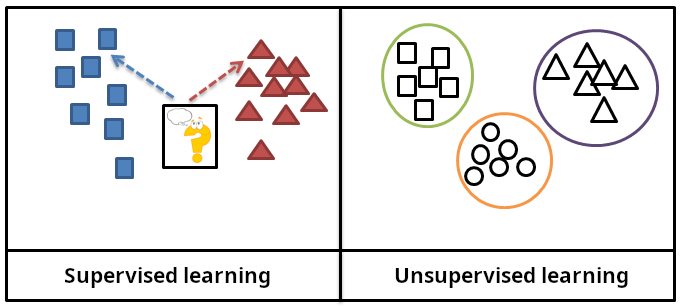
\includegraphics[width=0.7\textwidth]{images/teori-supervised.png}}
\caption{Perbandingan \textit{supervised learning}
 (data berlabel, ada acuan jawaban) dan \textit{unsupervised learning} (data tanpa label, mencari kelompok sendiri) \cite{wikipedia-supervised}.}
\label{fig:sup-unsup}
\end{figure}


\section{Forecasting}
\textit{Forecasting} adalah proses memperkirakan keadaan di masa depan dengan menguji pola pada data masa lalu \cite{vimala2022,hyndman2021}. Hasil ramalan membantu pengambilan keputusan, misalnya menentukan jumlah stok barang atau perencanaan kapasitas. Ramalan bisa bersifat kualitatif, seperti perkiraan bahwa besok cuaca cerah, atau kuantitatif berupa angka. Praktikum ini mengerjakan jenis yang kedua karena targetnya berupa nilai kontinu.

Peramalan deret waktu berbeda dari regresi biasa karena urutan waktu data tidak boleh diacak. Nilai hari ini bergantung pada nilai beberapa hari sebelumnya, sehingga susunan data saat pelatihan harus tetap kronologis. Modul membedakan dua jenis peramalan berdasarkan jarak prediksinya:
\begin{itemize}
    \item \textbf{One-step forecast:} model memprediksi satu nilai untuk satu langkah waktu berikutnya.
    \item \textbf{Multi-step forecast:} model memprediksi beberapa langkah waktu sekaligus, misalnya dua hari ke depan seperti pada tugas praktikum ini.
\end{itemize}
Perbandingan kedua jenis peramalan ini tampak pada Gambar~\ref{fig:one-multi}, sedangkan komponen penyusun deret waktu ditunjukkan pada Gambar~\ref{fig:komponen-ts}.

\begin{figure}[H]
\centering
\fbox{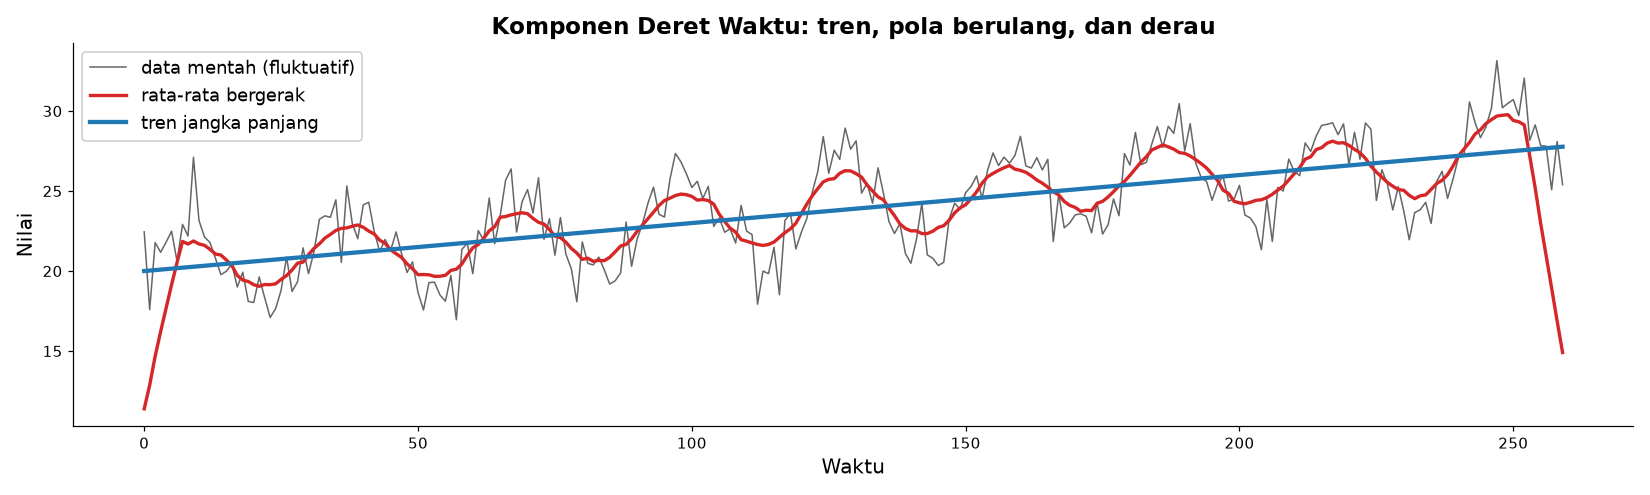
\includegraphics[width=0.6\textwidth]{images/teori-timeseries.png}}
\caption{Komponen deret waktu: data mentah yang berfluktuasi, rata-rata bergerak sebagai penghalus, dan tren jangka panjang.}
\label{fig:komponen-ts}
\end{figure}

\begin{figure}[H]
\centering
\fbox{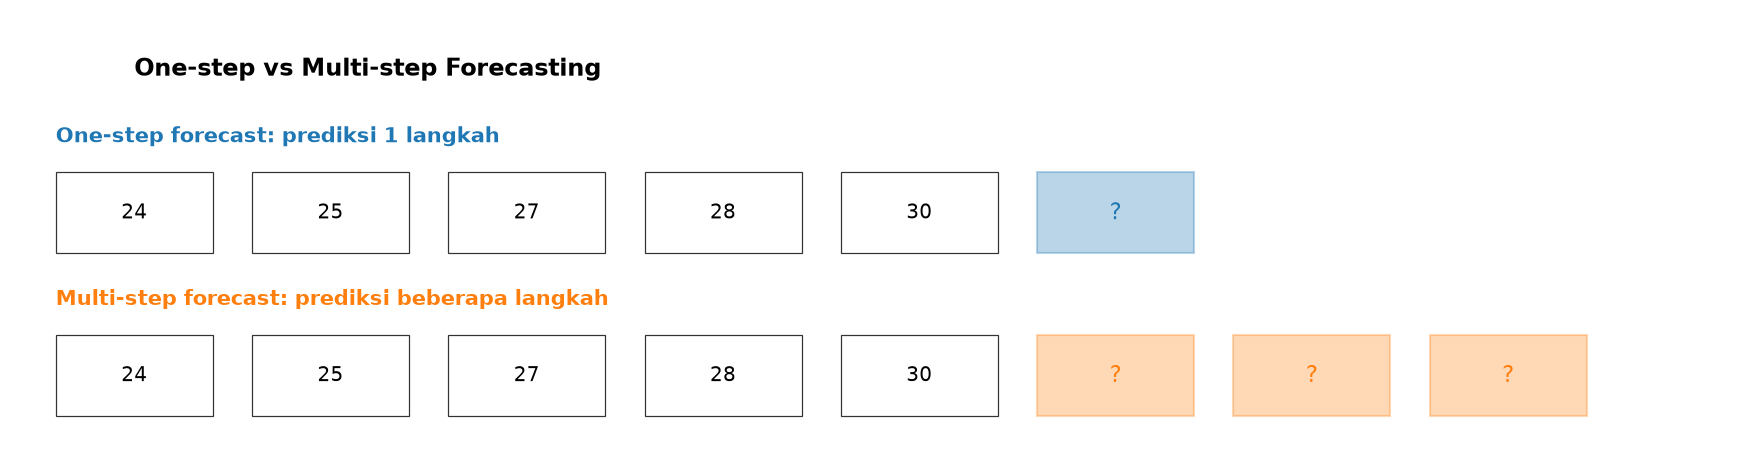
\includegraphics[width=0.9\textwidth]{images/teori-04-one-vs-multistep.png}}
\caption{Perbandingan \textit{one-step forecast}
 (satu langkah ke depan) dan \textit{multi-step forecast} (beberapa langkah sekaligus).}
\label{fig:one-multi}
\end{figure}


\section{Sliding Window}
Untuk mengubah deret waktu menjadi format \textit{supervised learning}, dipakai teknik \textit{sliding window}. Jendela berukuran tetap digeser satu langkah demi satu langkah sepanjang deret, sehingga setiap posisi menghasilkan satu pasangan masukan dan target \cite{wikipedia-sliding,hyndman2021}. Misalnya dengan ukuran jendela 7, nilai tujuh hari pertama menjadi masukan dan nilai hari ke-8 menjadi target, lalu jendela digeser satu hari untuk membentuk pasangan berikutnya.

Pendekatan ini dipakai karena algoritma regresi pada umumnya menerima tabel fitur, bukan urutan. Setelah diubah, pola urutan waktu bisa dipelajari oleh model seperti Linear Regression, Decision Tree, maupun Random Forest. Cara kerja penggeseran jendela ini diilustrasikan pada Gambar~\ref{fig:sliding}.

\begin{figure}[H]
\centering
\fbox{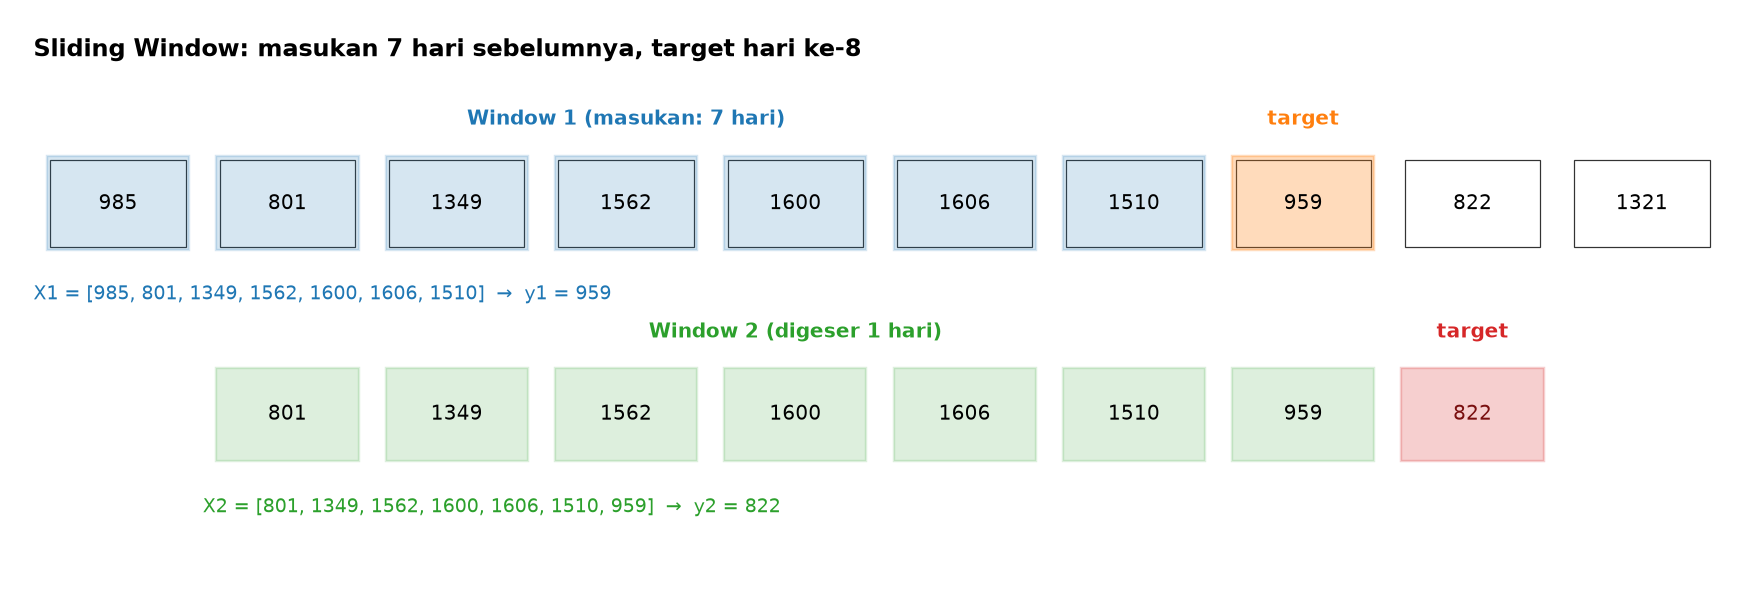
\includegraphics[width=0.95\textwidth]{images/teori-01-sliding-window.png}}
\caption{Teknik \textit{sliding window}
: jendela berisi tujuh nilai menjadi masukan, nilai hari ke-8 menjadi target, lalu jendela digeser satu hari untuk membentuk pasangan berikutnya.}
\label{fig:sliding}
\end{figure}


\section{Feature Engineering: Fitur Statistik}
Fitur statistik ditambahkan pada tiap jendela agar model mendapat gambaran distribusi data di dalamnya. Modul menyebut delapan fitur: nilai minimum, maksimum, selisih maksimum dan minimum, rata-rata, standar deviasi, median, kurtosis, dan skewness. Min, max, dan selisih menggambarkan rentang nilai; mean, median, dan standar deviasi menggambarkan pusat dan sebaran; sedangkan kurtosis dan skewness menggambarkan bentuk distribusi \cite{wikipedia-feature,scipy-kurtosis,scipy-skew}. Dengan tujuh nilai mentah ditambah delapan fitur statistik, satu sampel menjadi 15 fitur. Contoh perhitungan fitur-fitur ini pada satu jendela ditunjukkan pada Gambar~\ref{fig:fitur-stat}.

\begin{figure}[H]
\centering
\fbox{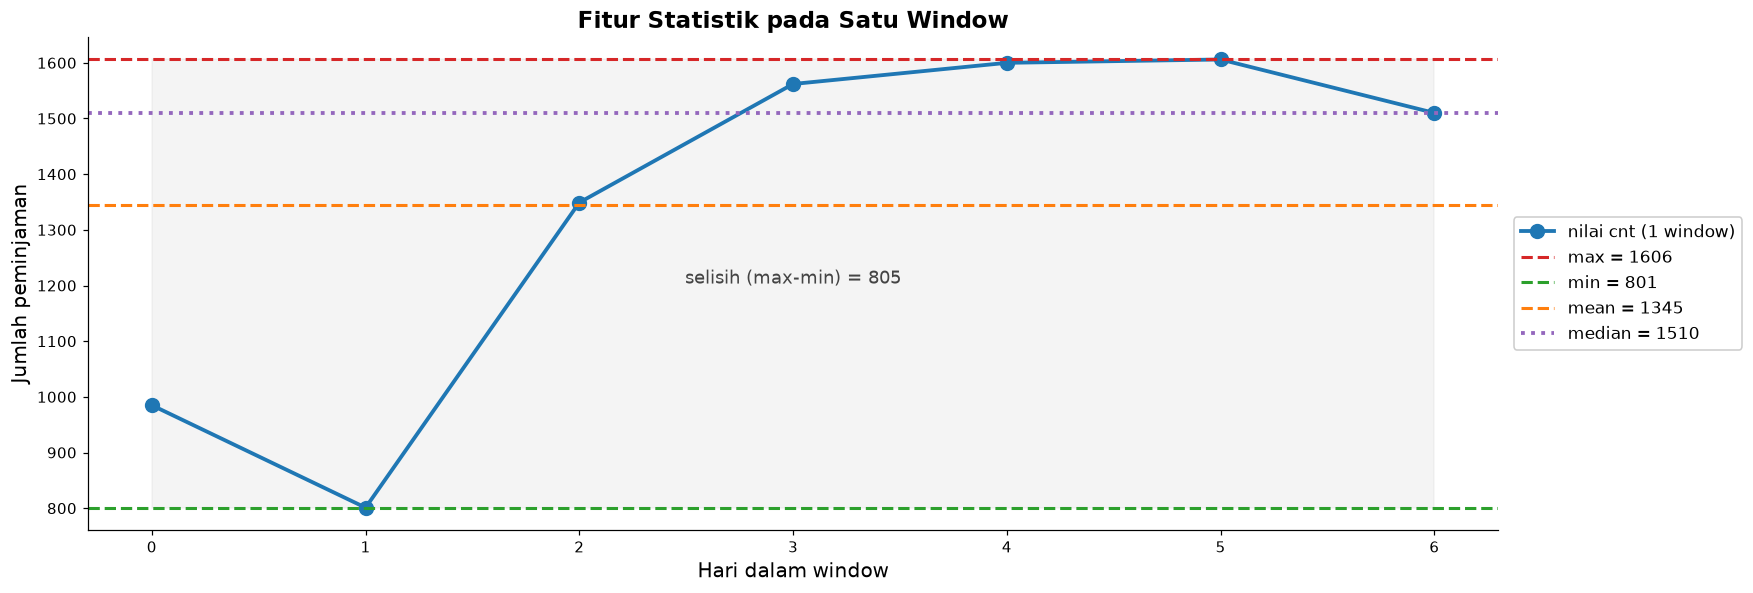
\includegraphics[width=0.95\textwidth]{images/teori-03-fitur-statistik.png}}
\caption{Fitur statistik pada satu jendela: minimum, maksimum, selisih, rata-rata, dan median tampak sebagai garis acuan terhadap deret harian. Standar deviasi, kurtosis, dan skewness juga dihitung sebagai angka, tetapi tidak digambar karena skalanya berbeda.}
\label{fig:fitur-stat}
\end{figure}


\section{Algoritma Machine Learning}
Modul memakai lima algoritma regresi. Linear Regression tidak dipakai di sini karena modul menyoroti lima model berikut.

\subsection{Multilayer Perceptron (Neural Network)}
MLPRegressor adalah jaringan saraf tiruan berlapis yang tersusun dari unit masukan, satu atau lebih lapisan tersembunyi, dan unit keluaran. Setiap koneksi punya bobot yang diperbarui lewat \textit{backpropagation} untuk menekan kesalahan prediksi \cite{sklearn-mlp,wikipedia-mlp}. Jaringan ini cukup lentur menangkap hubungan non-linear, tetapi hasilnya bisa berbeda tiap kali dijalankan bila \texttt{random\_state} tidak dikunci. Karena itu modul memakai \texttt{random\_state=42} agar hasilnya dapat direproduksi. Struktur jaringan yang dipakai tampak pada Gambar~\ref{fig:mlp}.

\begin{figure}[H]
\centering
\fbox{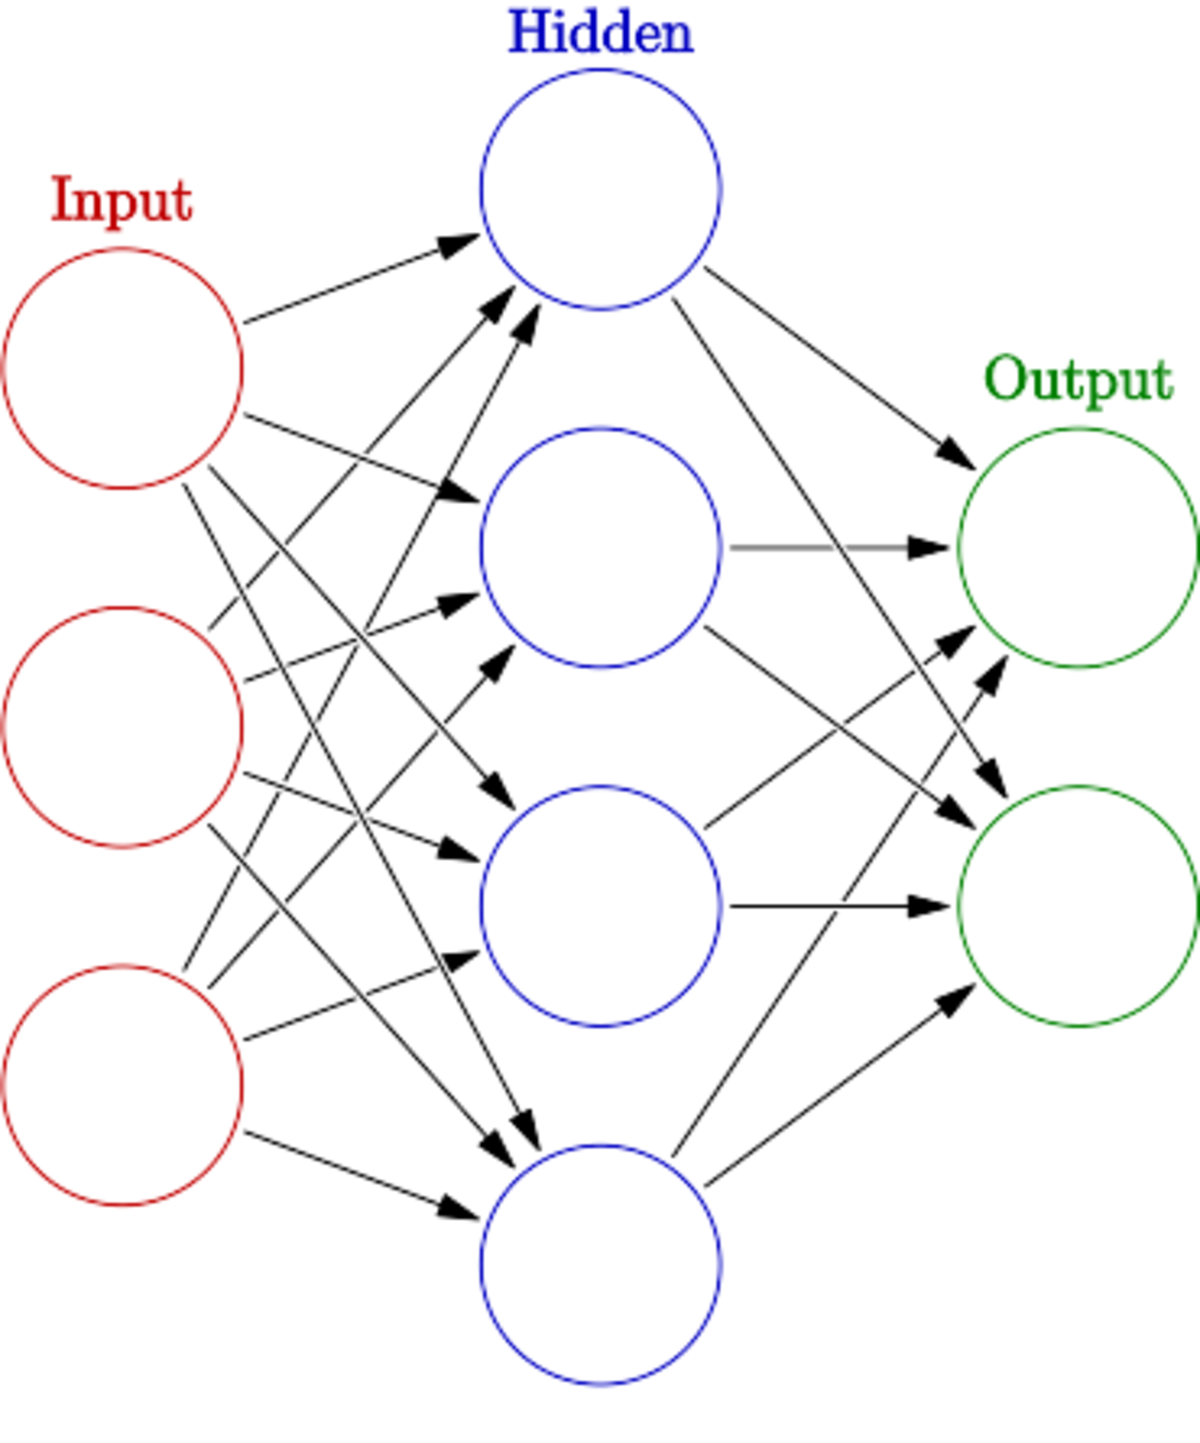
\includegraphics[width=0.5\textwidth]{images/teori-mlp.png}}
\caption{Arsitektur \textit{multilayer perceptron}: lapisan masukan, lapisan tersembunyi, dan lapisan keluaran yang terhubung penuh \cite{wikipedia-mlp}.}
\label{fig:mlp}
\end{figure}


\subsection{K-Nearest Neighbors (KNN)}
KNeighborsRegressor memprediksi nilai sebuah titik dengan merata-ratakan target dari $k$ tetangga terdekatnya \cite{sklearn-knn,wikipedia-knn}. Model ini tidak membangun persamaan saat pelatihan, seluruh data latih disimpan dan dibandingkan saat prediksi. Nilai $k$ bawaan adalah 5. Kelebihan KNN adalah kesederhanaannya, sedangkan kelemahannya ia sensitif terhadap skala fitur dan menjadi lambat ketika data latih membesar. Ilustrasi cara kerja KNN ditunjukkan pada Gambar~\ref{fig:knn}.

\begin{figure}[H]
\centering
\fbox{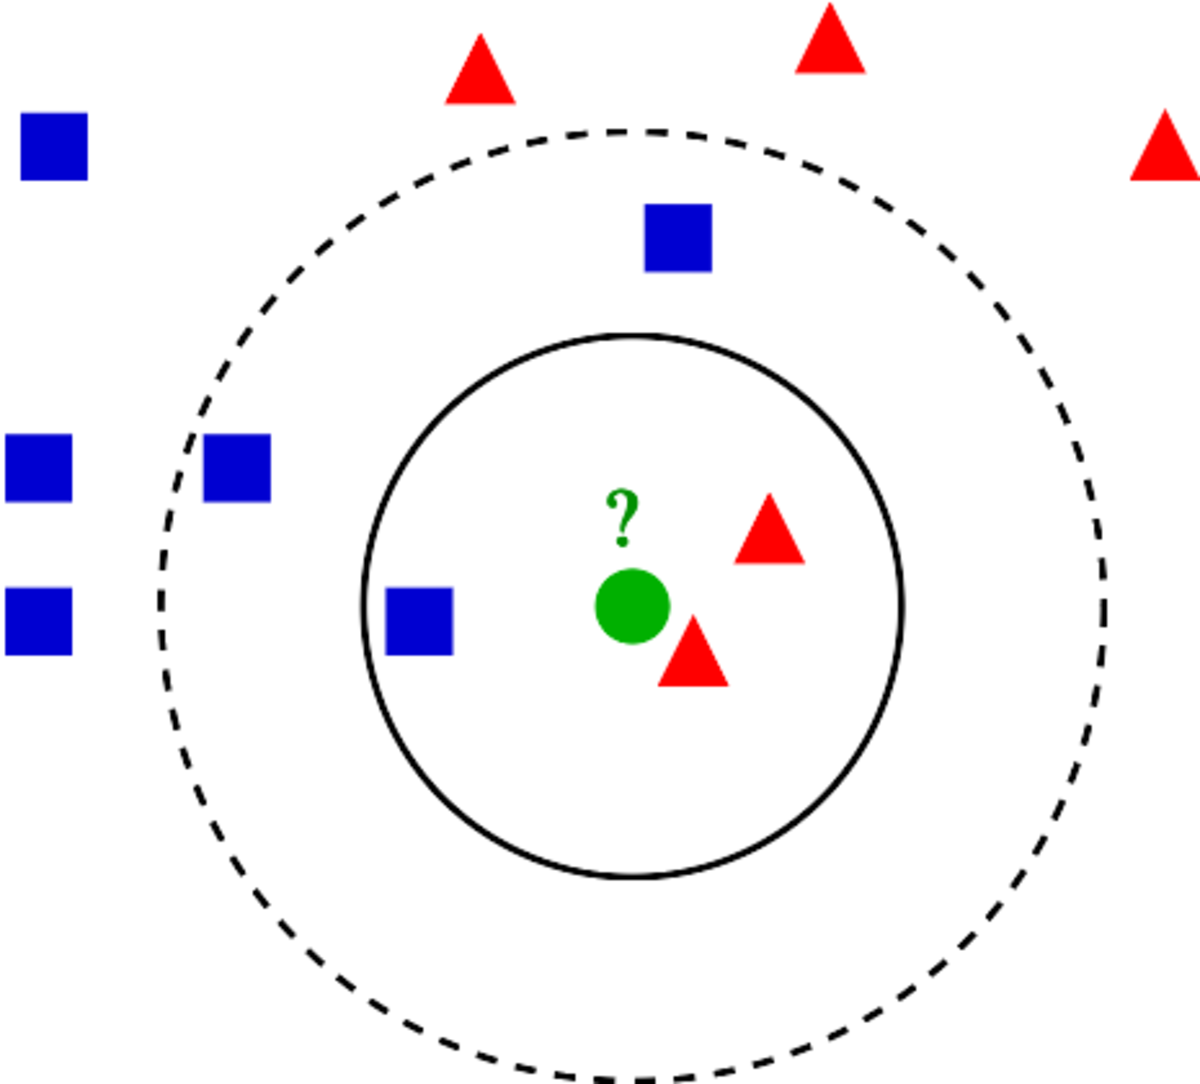
\includegraphics[width=0.55\textwidth]{images/teori-knn.png}}
\caption{Konsep KNN: titik uji (tanda tanya) diklasifikasikan berdasarkan mayoritas $k$ tetangga terdekat, di mana nilai $k$ memengaruhi hasilnya \cite{wikipedia-knn}.}
\label{fig:knn}
\end{figure}


\subsection{Decision Tree}
DecisionTreeRegressor membagi data secara rekursif berdasarkan titik pemisah yang paling menurunkan kesalahan, biasanya diukur dengan \textit{Mean Squared Error}. Setiap daun berisi nilai prediksi berupa rata-rata target di dalamnya \cite{sklearn-tree,wikipedia-dt}. Pohon tunggal mudah dibaca, tetapi rawan \textit{overfitting} karena bisa tumbuh terlalu dalam mengikuti data latih. Contoh pohon keputusan dan gejala \textit{overfitting} masing-masing tampak pada Gambar~\ref{fig:dt} dan Gambar~\ref{fig:overfit}.

\begin{figure}[H]
\centering
\fbox{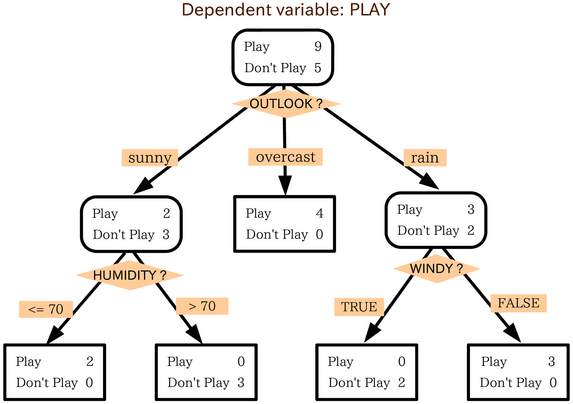
\includegraphics[width=0.7\textwidth]{images/teori-decision-tree.png}}
\caption{Contoh pohon keputusan untuk memprediksi keputusan bermain berdasarkan atribut cuaca \cite{wikipedia-dt}.}
\label{fig:dt}
\end{figure}

\begin{figure}[H]
\centering
\fbox{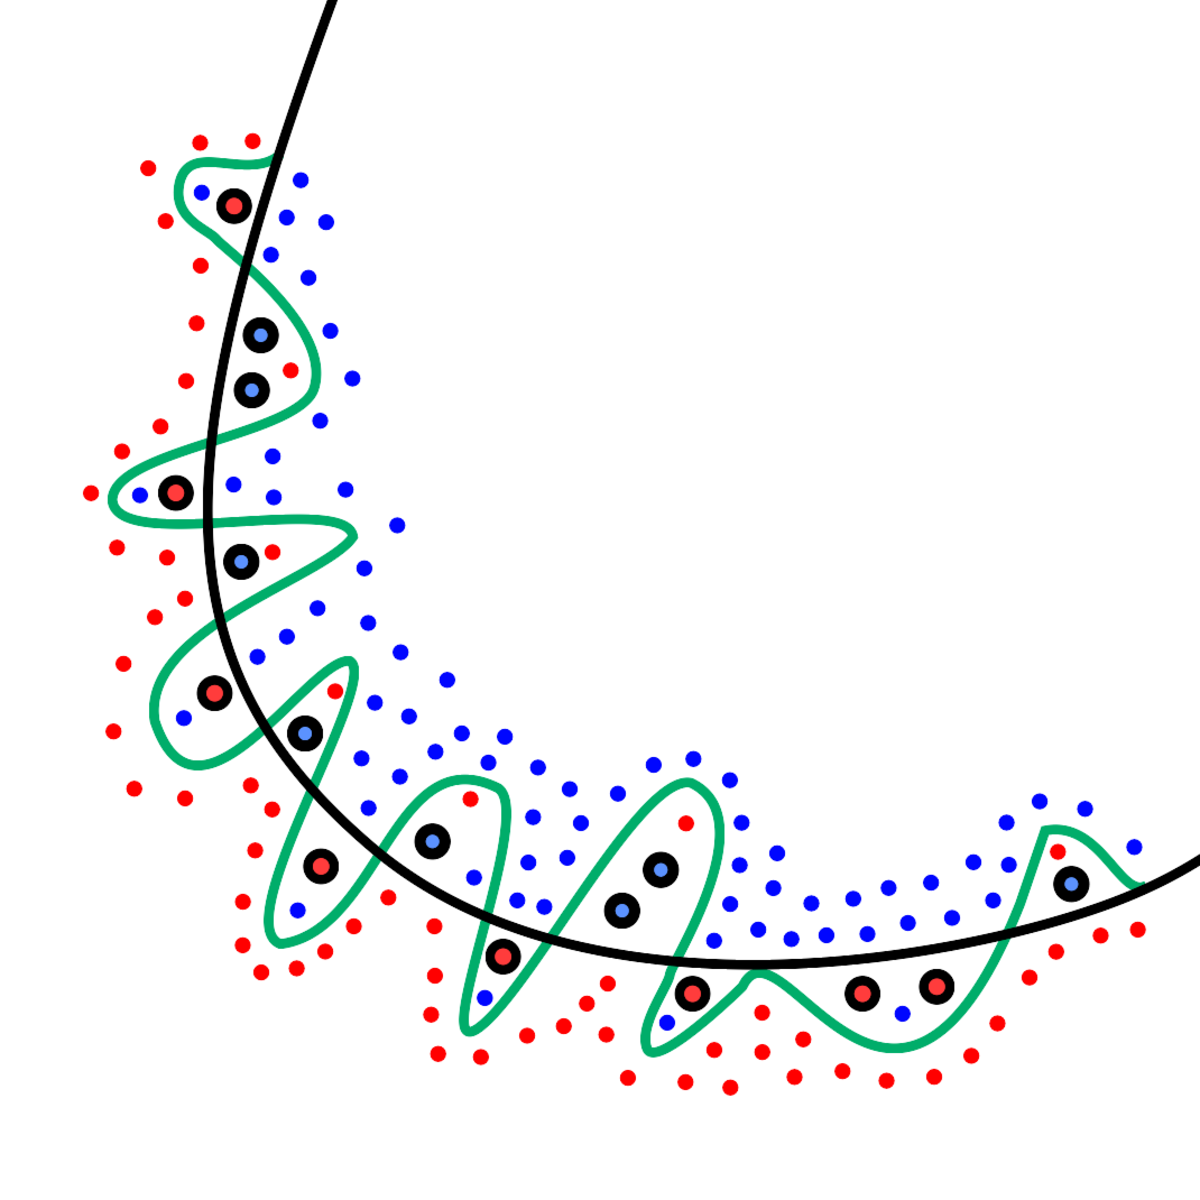
\includegraphics[width=0.5\textwidth]{images/teori-overfitting.png}}
\caption{Ilustrasi \textit{overfitting}: model terlalu mengikuti titik data latih sehingga kehilangan kemampuan generalisasi \cite{wikipedia-overfitting}.}
\label{fig:overfit}
\end{figure}


\subsection{Support Vector Regression (SVR)}
SVR mencari fungsi yang menyimpang paling jauh sebesar $\varepsilon$ dari target, sambil meminimalkan kompleksitas model \cite{sklearn-svr,wikipedia-svm}. Titik data yang berada di dalam batas $\varepsilon$ diabaikan dari fungsi biaya, sehingga SVR toleran terhadap derau kecil. Karena bekerja dengan jarak, fitur sebaiknya dinormalisasi lebih dulu agar tiap variabel memberi kontribusi seimbang. Konsep margin pada SVM ditunjukkan pada Gambar~\ref{fig:svr}.

\begin{figure}[H]
\centering
\fbox{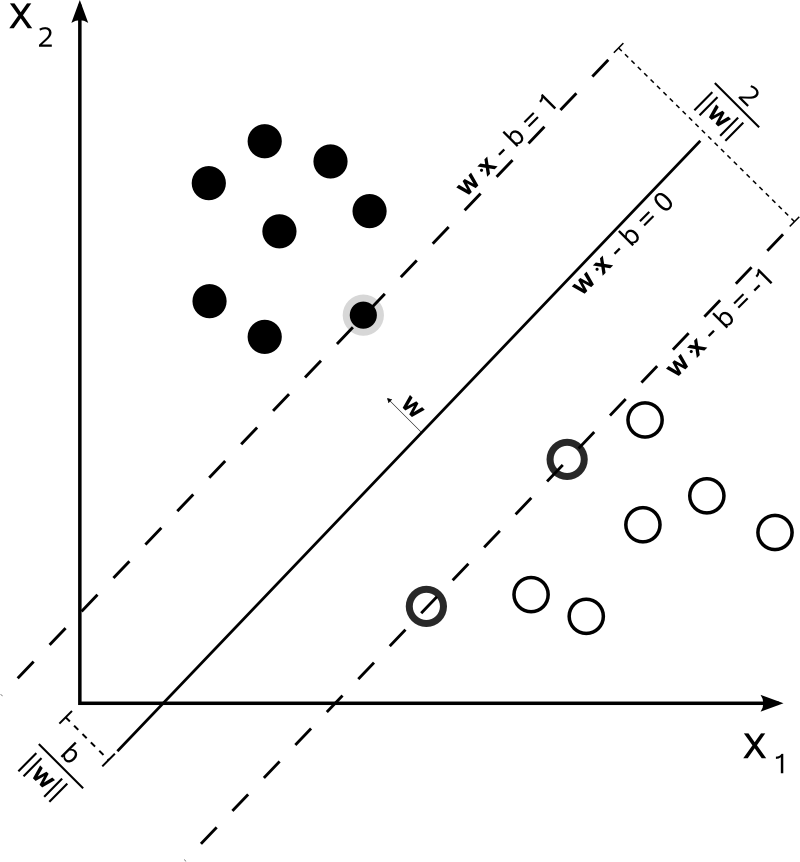
\includegraphics[width=0.5\textwidth]{images/teori-svr.png}}
\caption{Konsep margin maksimum pada Support Vector: garis pemisah optimal dan \textit{support vector} yang menentukan posisinya \cite{wikipedia-svm}.}
\label{fig:svr}
\end{figure}


\subsection{Random Forest}
RandomForestRegressor membangun banyak pohon keputusan dari sampel \textit{bootstrap} dan subset fitur acak, lalu merata-ratakan prediksinya \cite{sklearn-ensemble,wikipedia-rf}. Cara ini meredam kelemahan pohon tunggal, sehingga hasilnya lebih stabil dan tidak mudah \textit{overfitting}. Harganya adalah waktu latih dan kebutuhan memori yang lebih besar. Skema penggabungan hasil antar pohon tampak pada Gambar~\ref{fig:rf}.

\begin{figure}[H]
\centering
\fbox{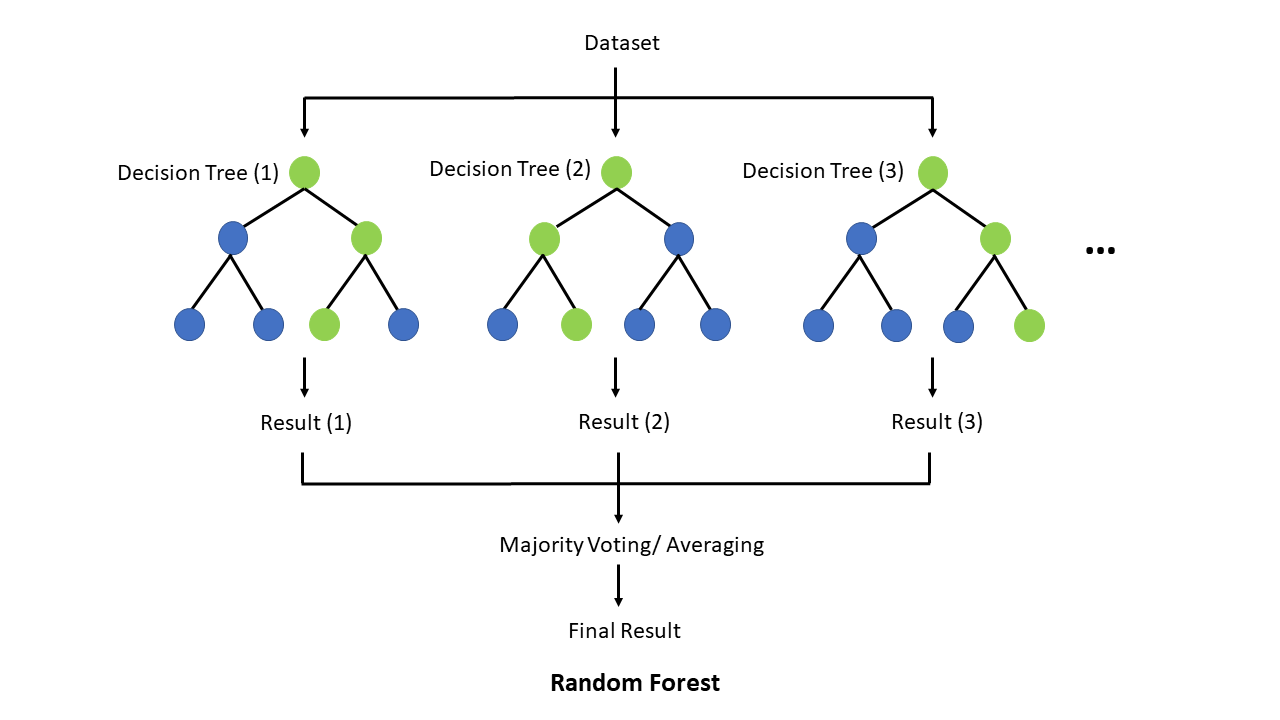
\includegraphics[width=0.8\textwidth]{images/teori-random-forest.png}}
\caption{Skema \textit{random forest}: beberapa pohon keputusan dibangun lalu hasilnya digabung melalui pemungutan suara atau rata-rata \cite{wikipedia-rf}.}
\label{fig:rf}
\end{figure}


\section{Metrik Evaluasi}

\subsection{Root Mean Squared Error (RMSE)}
RMSE mengukur rata-rata jarak antara nilai prediksi dan nilai aktual, dengan penalti lebih besar pada kesalahan yang besar. RMSE adalah akar dari \textit{Mean Squared Error}, sehingga satuannya sama dengan satuan target \cite{sklearn-metrics,chai2014}.
\begin{equation}
RMSE = \sqrt{\frac{1}{n}\sum_{i=1}^{n}(y_{pred,i} - y_{true,i})^2}
\end{equation}
Semakin kecil RMSE, semakin akurat model. Karena kesalahan dikuadratkan, RMSE peka terhadap \textit{outlier}: satu prediksi yang jauh meleset akan menaikkan nilai RMSE cukup besar.

\subsection{Pearson Correlation Coefficient}
Koefisien korelasi Pearson ($r$) mengukur kekuatan dan arah hubungan linear antara nilai aktual dan nilai prediksi. Nilainya berkisar dari $-1$ sampai $1$. Nilai mendekati 1 berarti prediksi mengikuti pola aktual dengan arah yang sama, mendekati $-1$ berarti hubungannya berlawanan, dan mendekati 0 berarti tidak ada hubungan linear \cite{benesty2009,scipy-pearson}.
\begin{equation}
r = \frac{\sum (y_{true,i} - \bar{y}_{true})(y_{pred,i} - \bar{y}_{pred})}{\sqrt{\sum (y_{true,i} - \bar{y}_{true})^2 \sum (y_{pred,i} - \bar{y}_{pred})^2}}
\end{equation}
RMSE dan Pearson saling melengkapi. RMSE menunjukkan besar kesalahan, sedangkan Pearson menunjukkan seberapa baik bentuk pola prediksi menyerupai pola aktual. Rentang nilai koefisien korelasi ini digambarkan pada Gambar~\ref{fig:pearson}.

\begin{figure}[H]
\centering
\fbox{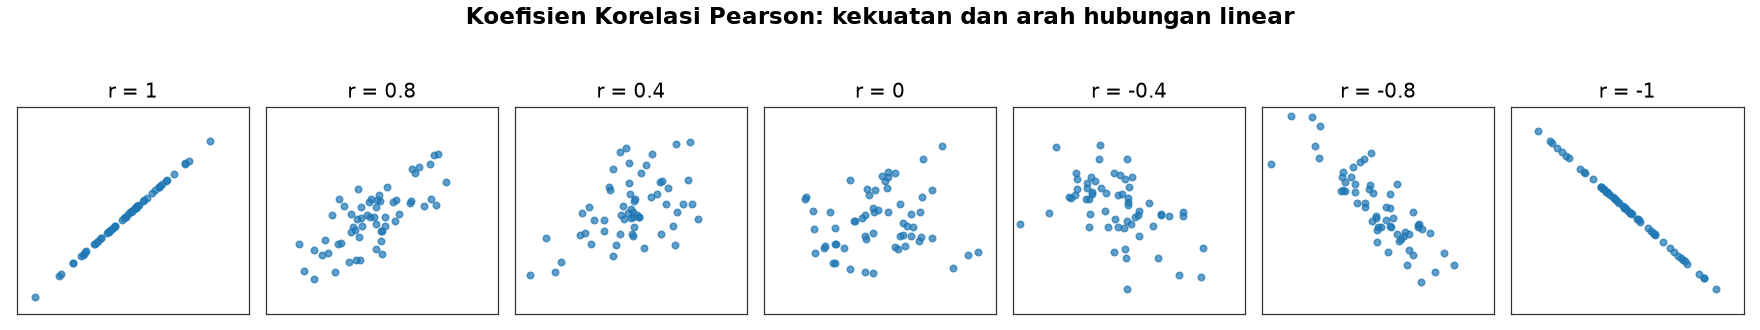
\includegraphics[width=0.95\textwidth]{images/teori-pearson.png}}
\caption{Nilai koefisien korelasi Pearson dari 1 sampai $-1$: tanda menunjukkan arah hubungan, sedangkan besar nilainya menunjukkan kekuatan hubungan linear.}
\label{fig:pearson}
\end{figure}


\section{Validasi dan Pencegahan Data Leakage}
Data dibagi menjadi bagian latih dan bagian uji. Pada deret waktu, pembagian tidak boleh diacak karena akan membuat model "melihat" masa depan. Modul memakai \texttt{shuffle=False} pada \texttt{train\_test\_split} agar 80\% data awal menjadi latih dan 20\% data akhir menjadi uji \cite{sklearn-split}. Normalisasi juga di-\textit{fit} hanya pada data latih, lalu diterapkan ke data uji, supaya informasi dari data uji tidak bocor ke proses pelatihan \cite{sklearn-preprocessing}. Skema pembagian data ini ditunjukkan pada Gambar~\ref{fig:split}.

\begin{figure}[H]
\centering
\fbox{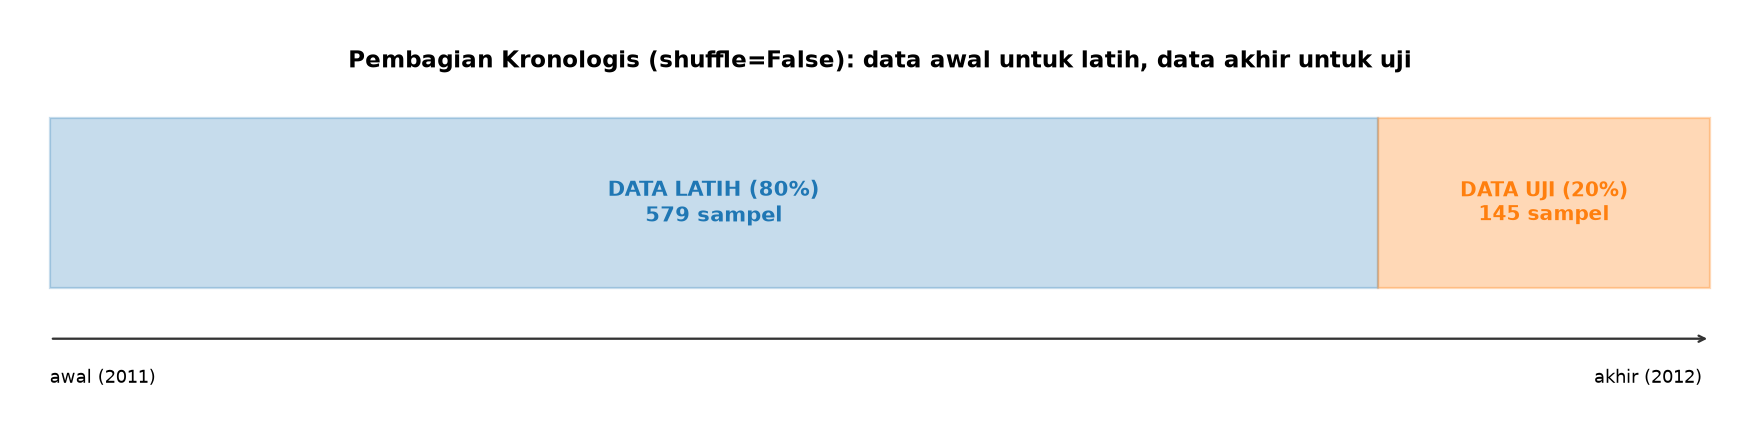
\includegraphics[width=0.9\textwidth]{images/teori-02-split-kronologis.png}}
\caption{Pembagian data kronologis dengan \texttt{shuffle=False}: 80\% data awal untuk latih dan 20\% data akhir untuk uji.}
\label{fig:split}
\end{figure}


\clearpage

\chapter[\tocboldsection{Hasil dan Pembahasan}]{Hasil dan Pembahasan}

\section{Percobaan Latihan Praktikum}
Bagian ini mendokumentasikan percobaan \textit{forecasting} sesuai langkah pada Modul Pertemuan 5. Dataset yang dipakai adalah \textit{Bike Sharing Dataset} \cite{kaggle-bike}, yang berisi catatan peminjaman sepeda harian beserta kondisi cuaca. Saya memuat data dari mirror GitHub \cite{bike-mirror} agar bisa langsung dibaca dengan \texttt{pd.read\_csv()} tanpa unduhan manual. Notebook yang saya gunakan dapat dijalankan langsung melalui Google Colab pada tautan berikut: \url{https://colab.research.google.com/github/hafidzrizqullahprasetya/PPD/blob/main/pertemuan-5/praktikum-5-forecasting.ipynb} \cite{colab-notebook}, dan salinannya juga tersedia pada repositori ini sebagai \texttt{praktikum-5-forecasting.ipynb}.

\subsection{Alat dan Bahan}
Sesuai Modul 5.3, alat dan bahan yang saya gunakan adalah:
\begin{itemize}
    \item \textbf{Perangkat keras:} laptop dengan RAM minimal 4 GB dan koneksi internet stabil.
    \item \textbf{Perangkat lunak:} Python~3 \cite{python-docs} dan lingkungan notebook (Google Colab atau Jupyter). Pustaka utama meliputi pandas \cite{pandas-docs}, NumPy \cite{numpy-docs}, Matplotlib \cite{matplotlib-docs}, Seaborn \cite{seaborn-docs}, Scikit-Learn \cite{sklearn-metrics,sklearn-preprocessing}, dan SciPy untuk perhitungan korelasi \cite{scipy-pearson}.
\end{itemize}

\subsection{Persiapan dan Impor Pustaka}
Saya mengimpor pustaka untuk manipulasi data, perhitungan numerik, visualisasi, pemodelan lima algoritma, serta metrik evaluasi. Blok impor juga memuat \texttt{pearsonr}, \texttt{kurtosis}, dan \texttt{skew} dari SciPy untuk evaluasi dan fitur statistik.

\begin{lstlisting}[style=pythonstyle,caption={Impor pustaka praktikum forecasting.}]
import numpy as np
import pandas as pd
from math import sqrt
import matplotlib.pyplot as plt
import seaborn as sns

from numpy import array
from scipy.stats import pearsonr, kurtosis, skew
from sklearn.metrics import mean_squared_error
from sklearn.model_selection import train_test_split
from sklearn.neural_network import MLPRegressor
from sklearn.neighbors import KNeighborsRegressor
from sklearn.tree import DecisionTreeRegressor
from sklearn.ensemble import RandomForestRegressor
from sklearn.svm import SVR
from sklearn.preprocessing import StandardScaler
\end{lstlisting}

\begin{figure}[H]
\centering
\customfbox{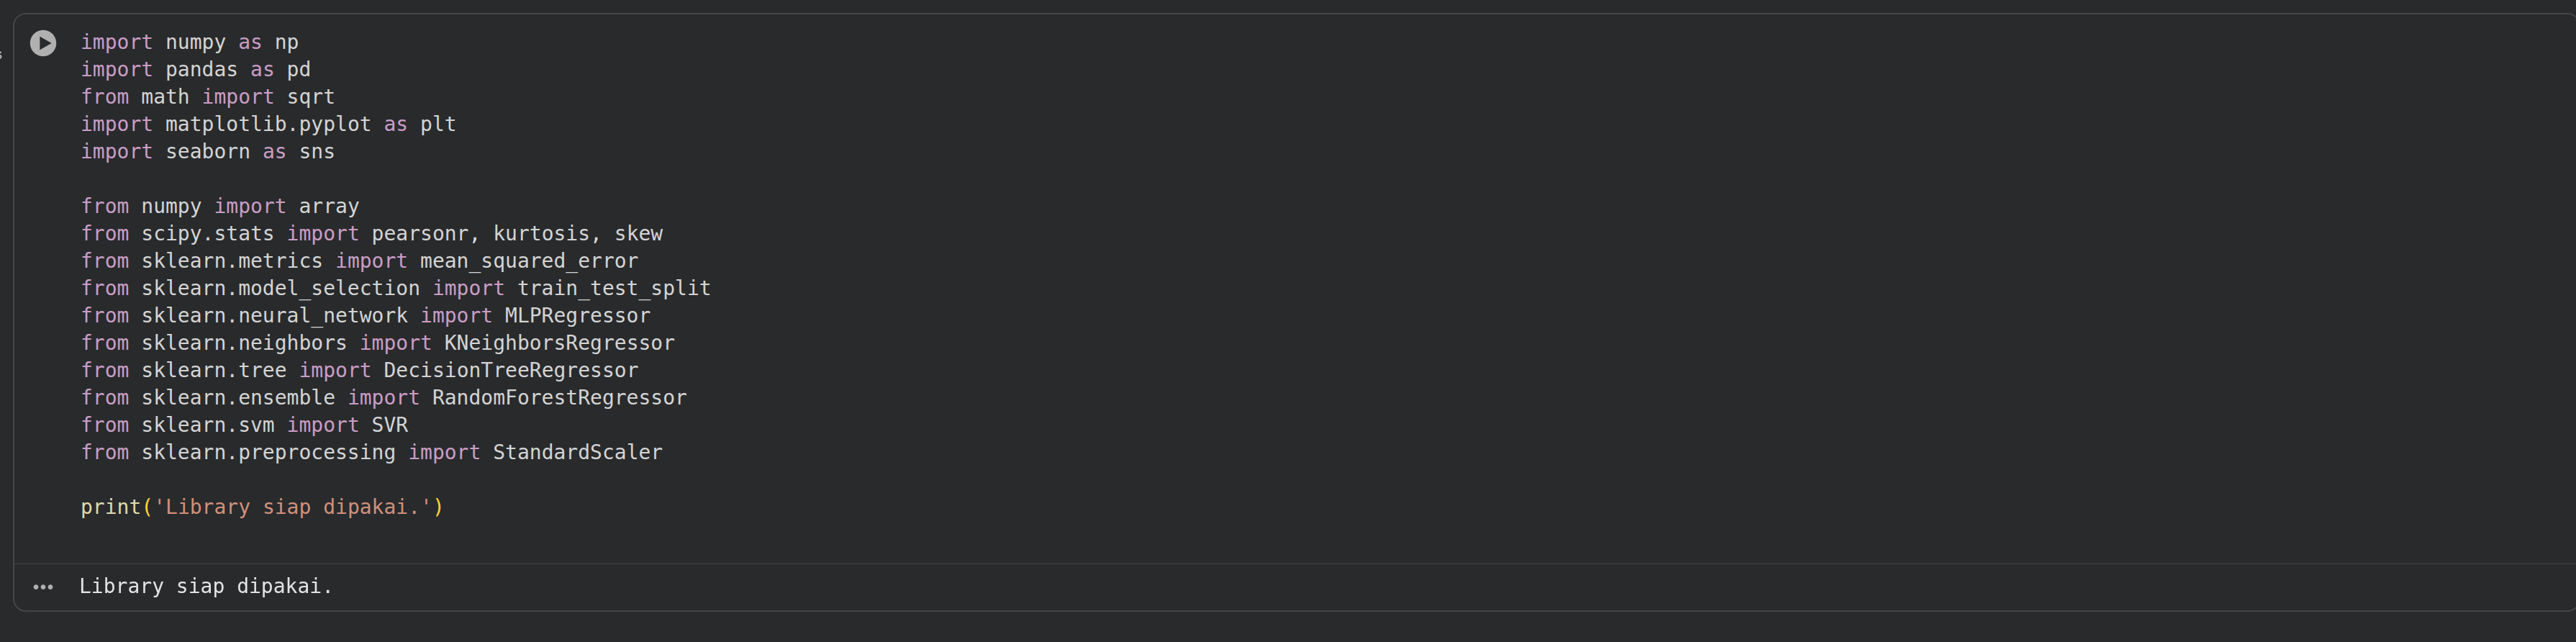
\includegraphics[width=0.95\textwidth]{images/t01-import.png}}
\caption{Blok impor pustaka yang dipakai sepanjang praktikum.}
\label{fig:import}
\end{figure}

\subsection{Fungsi Sliding Window}
Fungsi \texttt{split\_sequences} mengubah deret waktu menjadi pasangan masukan dan target. Untuk setiap posisi, ia mengambil \texttt{n\_steps\_in} baris sebagai masukan dan satu nilai pada \texttt{n\_steps\_out} langkah setelahnya sebagai target. Perulangan berhenti ketika jendela sudah melewati akhir data.

\begin{lstlisting}[style=pythonstyle,caption={Fungsi sliding window.}]
def split_sequences(sequences, n_steps_in, n_steps_out):
    X, y = list(), list()
    for i in range(len(sequences)):
        end_ix = i + n_steps_in
        out_end_ix = end_ix + n_steps_out
        if out_end_ix > len(sequences):
            break
        seq_x, seq_y = sequences[i:end_ix, :-1], sequences[out_end_ix - 1, -1]
        X.append(seq_x)
        y.append(seq_y)
    return array(X), array(y)
\end{lstlisting}

\subsection{Fungsi Fitur Statistik}
Fungsi \texttt{stats\_features} menghitung delapan nilai statistik pada setiap jendela, lalu menyambungkannya ke data mentah jendela tersebut. Hasilnya, satu sampel yang semula berisi tujuh nilai berubah menjadi 15 fitur.

\begin{lstlisting}[style=pythonstyle,caption={Fungsi fitur statistik.}]
def stats_features(input_data):
    inp = list()
    for i in range(len(input_data)):
        inp2 = input_data[i]
        min_val = float(np.min(inp2))
        max_val = float(np.max(inp2))
        diff = max_val - min_val
        std_val = float(np.std(inp2))
        mean_val = float(np.mean(inp2))
        median_val = float(np.median(inp2))
        kurt = float(kurtosis(inp2))
        sk = float(skew(inp2))
        for v in (min_val, max_val, diff, std_val, mean_val, median_val, kurt, sk):
            inp2 = np.append(inp2, v)
        inp = np.append(inp, inp2)
    return inp.reshape(len(input_data), -1)
\end{lstlisting}

\subsection{Memuat Dataset}
Dataset bike sharing berisi 731 baris dan 16 kolom, mencakup tanggal, kondisi cuaca, suhu, kelembapan, dan jumlah peminjaman pada kolom \texttt{cnt}.

\begin{lstlisting}[style=pythonstyle,caption={Memuat dataset bike sharing.}]
df = pd.read_csv('https://raw.githubusercontent.com/ganjar87/data_science_practice/main/bikesharing_day.csv')
print('shape:', df.shape)
df.head()
\end{lstlisting}

\begin{figure}[H]
\centering
\customfbox{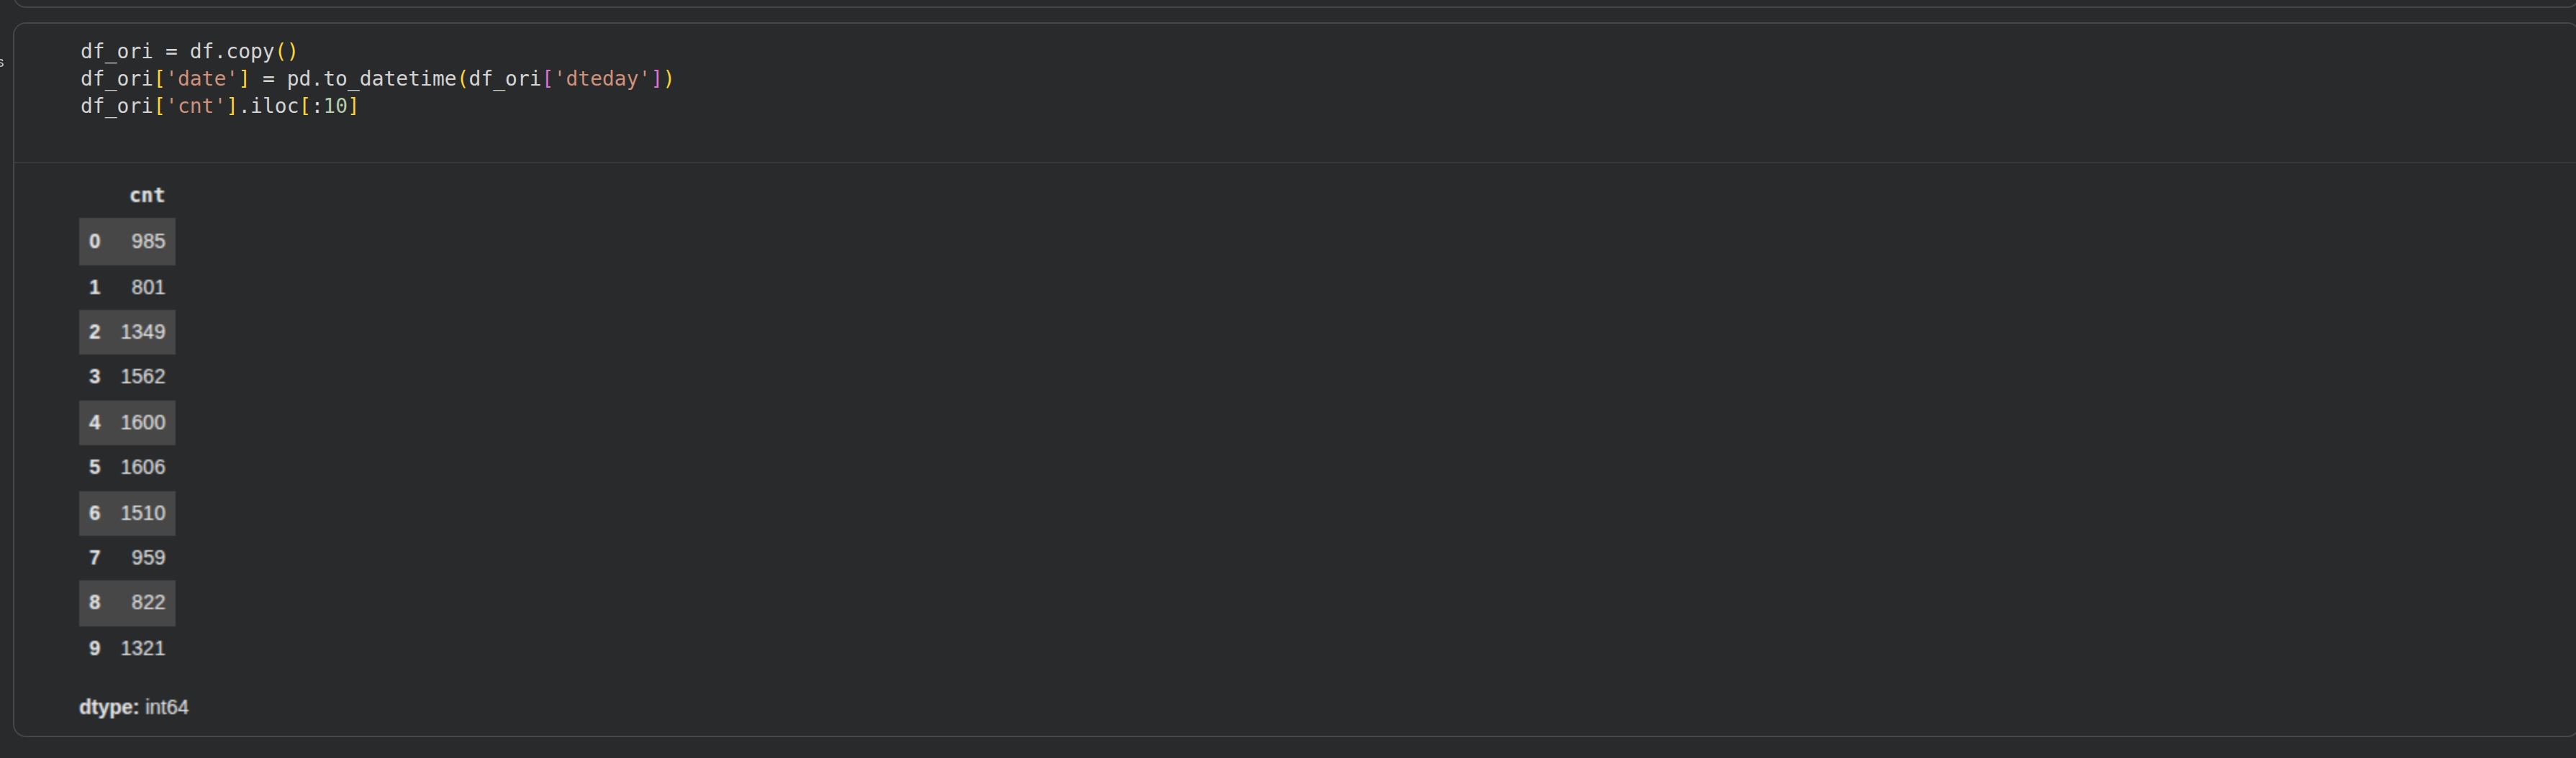
\includegraphics[width=0.98\textwidth]{images/t02-bike-head.png}}
\caption{Lima baris pertama dataset bike sharing: kolom \texttt{instant}, \texttt{dteday}, \texttt{season}, hingga \texttt{cnt}.}
\label{fig:bike-head}
\end{figure}

Kolom tanggal \texttt{dteday} saya ubah ke format datetime supaya bisa dipakai untuk sumbu waktu pada grafik.

\begin{lstlisting}[style=pythonstyle,caption={Konversi kolom tanggal dan cek sepuluh nilai target.}]
df_ori = df.copy()
df_ori['date'] = pd.to_datetime(df_ori['dteday'])
df_ori['cnt'].iloc[:10]
\end{lstlisting}

\begin{figure}[H]
\centering
\customfbox{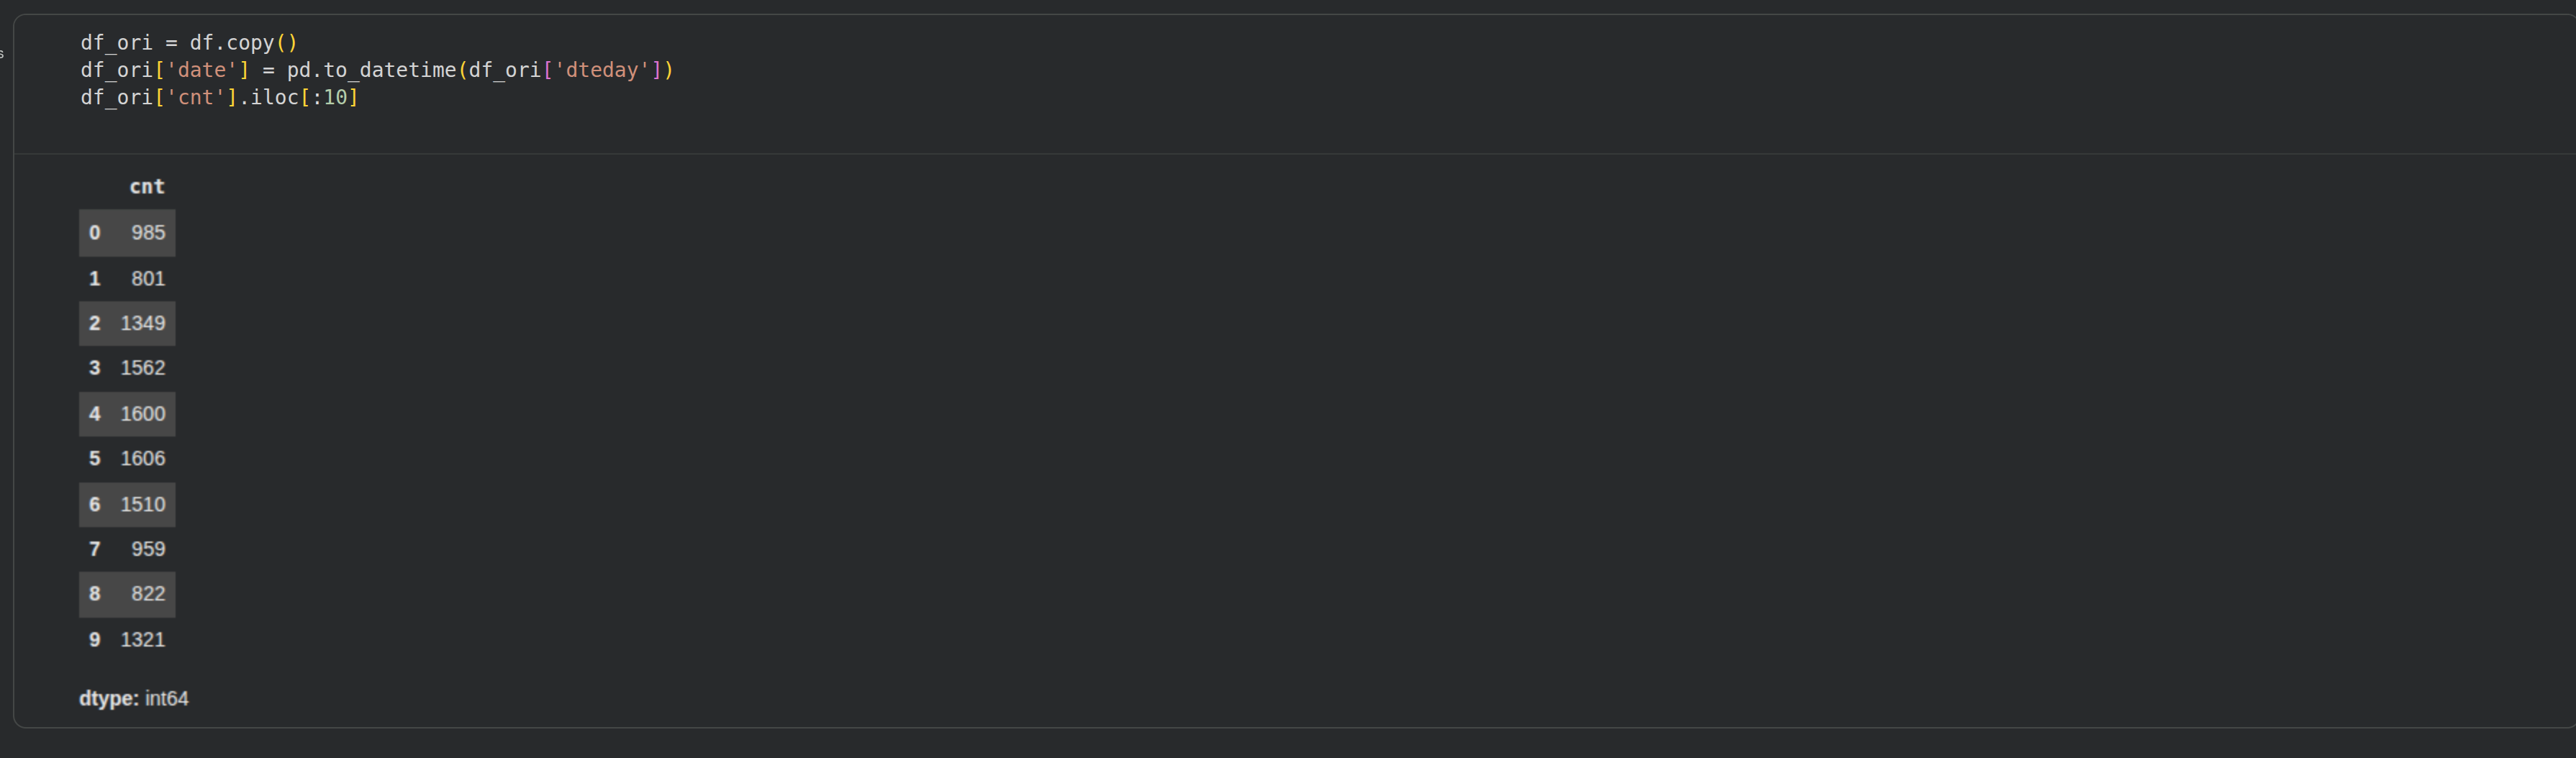
\includegraphics[width=0.55\textwidth]{images/t14-cnt.png}}
\caption{Sepuluh nilai pertama kolom target \texttt{cnt}: 985, 801, 1349, 1562, 1600, 1606, 1510, 959, 822, dan 1321.}
\label{fig:bike-cnt}
\end{figure}

\subsection{Membentuk Time Series dan Preprocessing}
Masukan dibentuk dari nilai \texttt{cnt} tujuh hari sebelumnya untuk memprediksi hari ke-8. Saya menduplikasi kolom \texttt{cnt} menjadi dua kolom karena fungsi \texttt{split\_sequences} memisahkan kolom terakhir sebagai target, sedangkan sisanya menjadi fitur. Data hasil jendela lalu dibagi 80:20 dengan \texttt{shuffle=False}, kemudian fitur statistik ditambahkan pada data latih dan data uji.

\begin{lstlisting}[style=pythonstyle,caption={Sliding window, split, dan penambahan fitur statistik.}]
df_X = df_ori[['cnt', 'cnt']]
in_seq = df_X.astype(float).values

n_steps_in, n_steps_out = 7, 1
X, y = split_sequences(in_seq, n_steps_in, n_steps_out)

n_input = X.shape[1] * X.shape[2]
X = X.reshape((X.shape[0], n_input))

X_train, X_test, y_train, y_test = train_test_split(
    X, y, test_size=0.2, random_state=42, shuffle=False)

X_train = stats_features(X_train)
X_test = stats_features(X_test)
\end{lstlisting}

\begin{figure}[H]
\centering
\customfbox{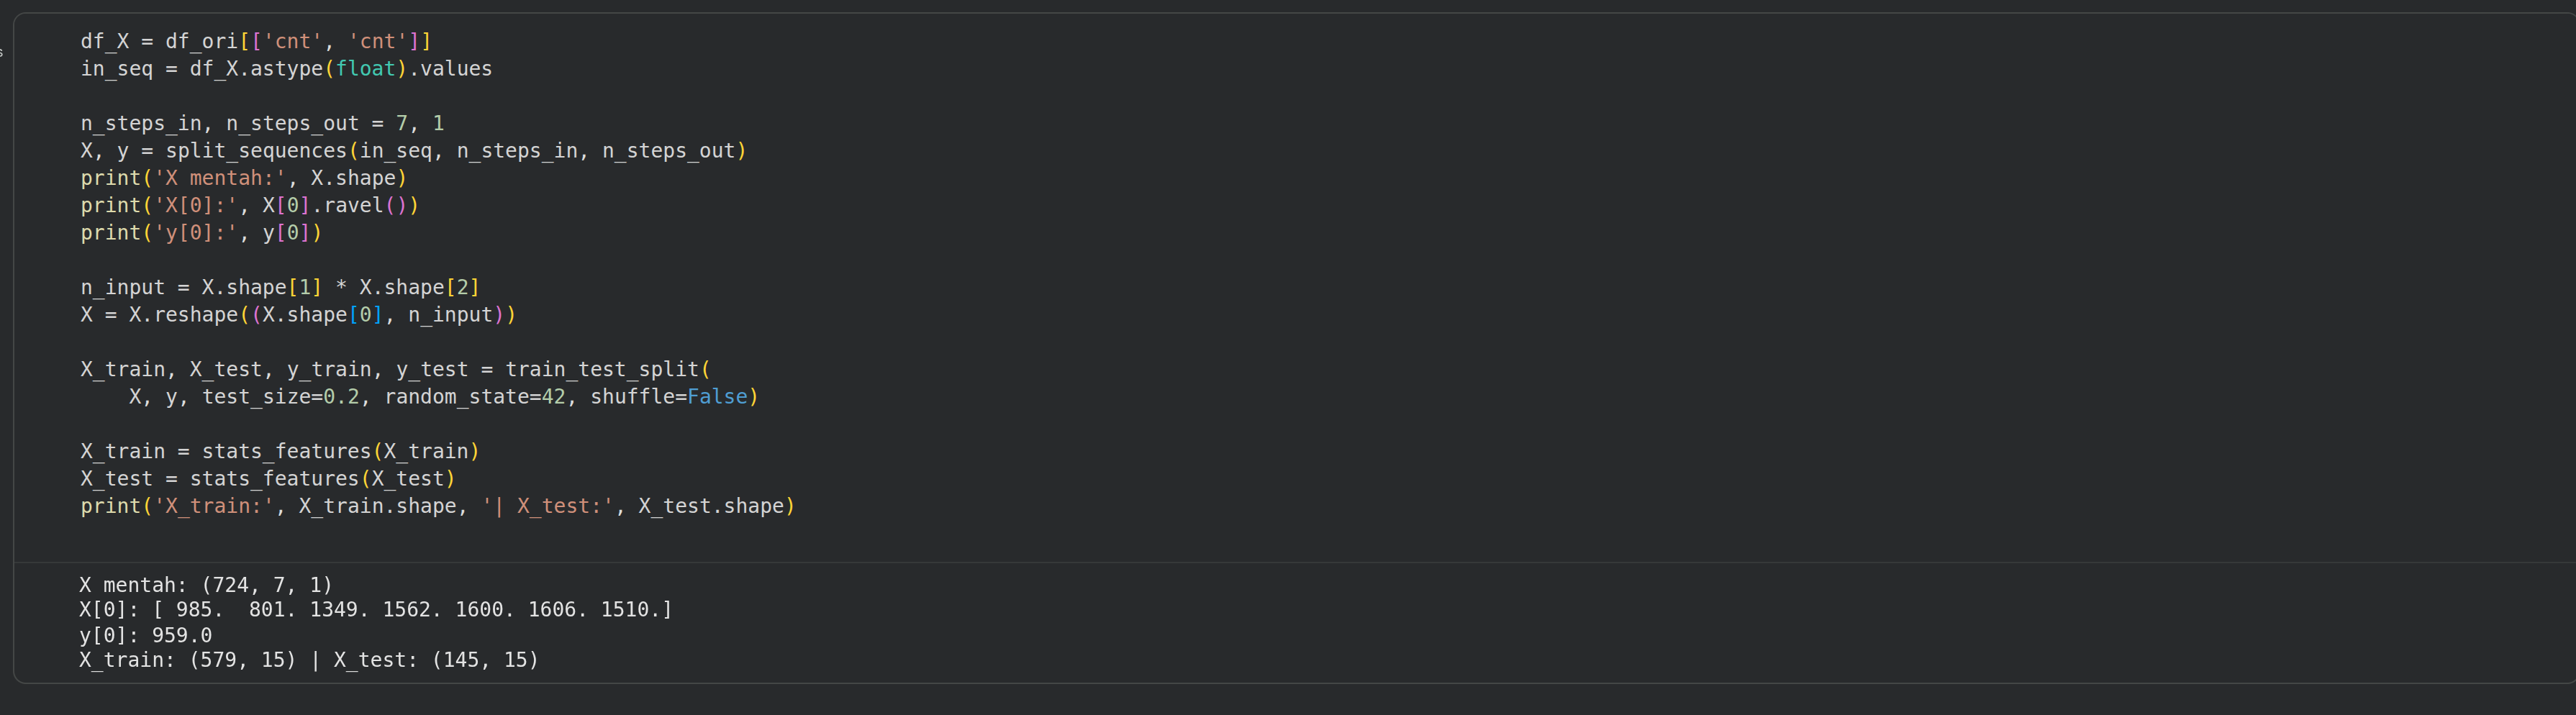
\includegraphics[width=0.6\textwidth]{images/t13-window.png}}
\caption{Hasil pembentukan jendela: 724 sampel dengan tujuh nilai masukan. Sampel pertama berisi tujuh hari awal, targetnya 959,0 pada hari ke-8.}
\label{fig:window}
\end{figure}

\begin{figure}[H]
\centering
\customfbox{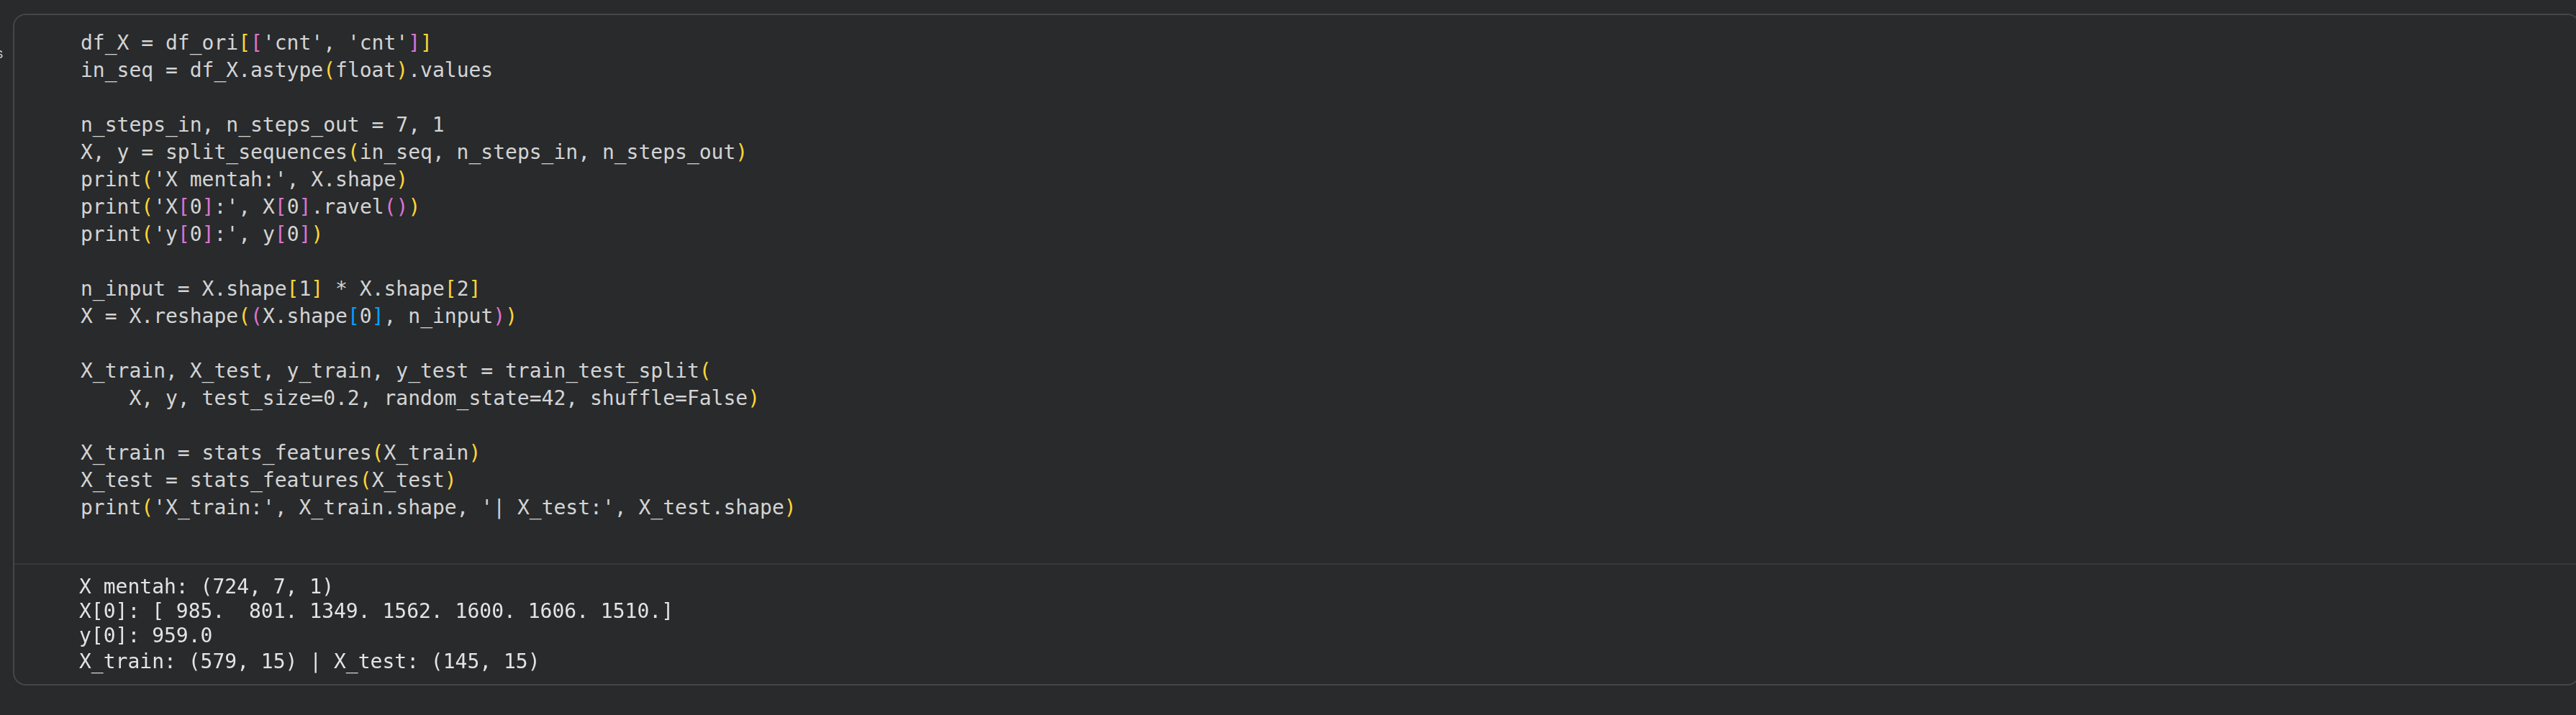
\includegraphics[width=0.6\textwidth]{images/t12-preprocess.png}}
\caption{Bentuk data setelah fitur statistik ditambahkan: 579 sampel latih dan 145 sampel uji, masing-masing dengan 15 fitur.}
\label{fig:preprocess}
\end{figure}

Jumlah 724 sampel berasal dari 731 baris dikurangi 7 hari yang tidak punya riwayat sebelumnya. Pembagian 80:20 menghasilkan 579 sampel latih dan 145 sampel uji, dan jumlah kolom bertambah dari 7 menjadi 15 setelah delapan fitur statistik disisipkan.

\subsection{Visualisasi Deret Waktu}
Sebelum melatih model, saya melihat pola deret waktu jumlah peminjaman sepeda untuk memahami sifat datanya.

\begin{lstlisting}[style=pythonstyle,caption={Visualisasi deret waktu jumlah peminjaman.}]
fig = plt.figure(figsize=(16, 5))
plt.plot(df_ori['date'], df_ori['cnt'])
plt.ylabel('# total rented bikes', fontsize=14)
plt.xlabel('Tanggal', fontsize=14)
plt.show()
\end{lstlisting}

\begin{figure}[H]
\centering
\customfbox{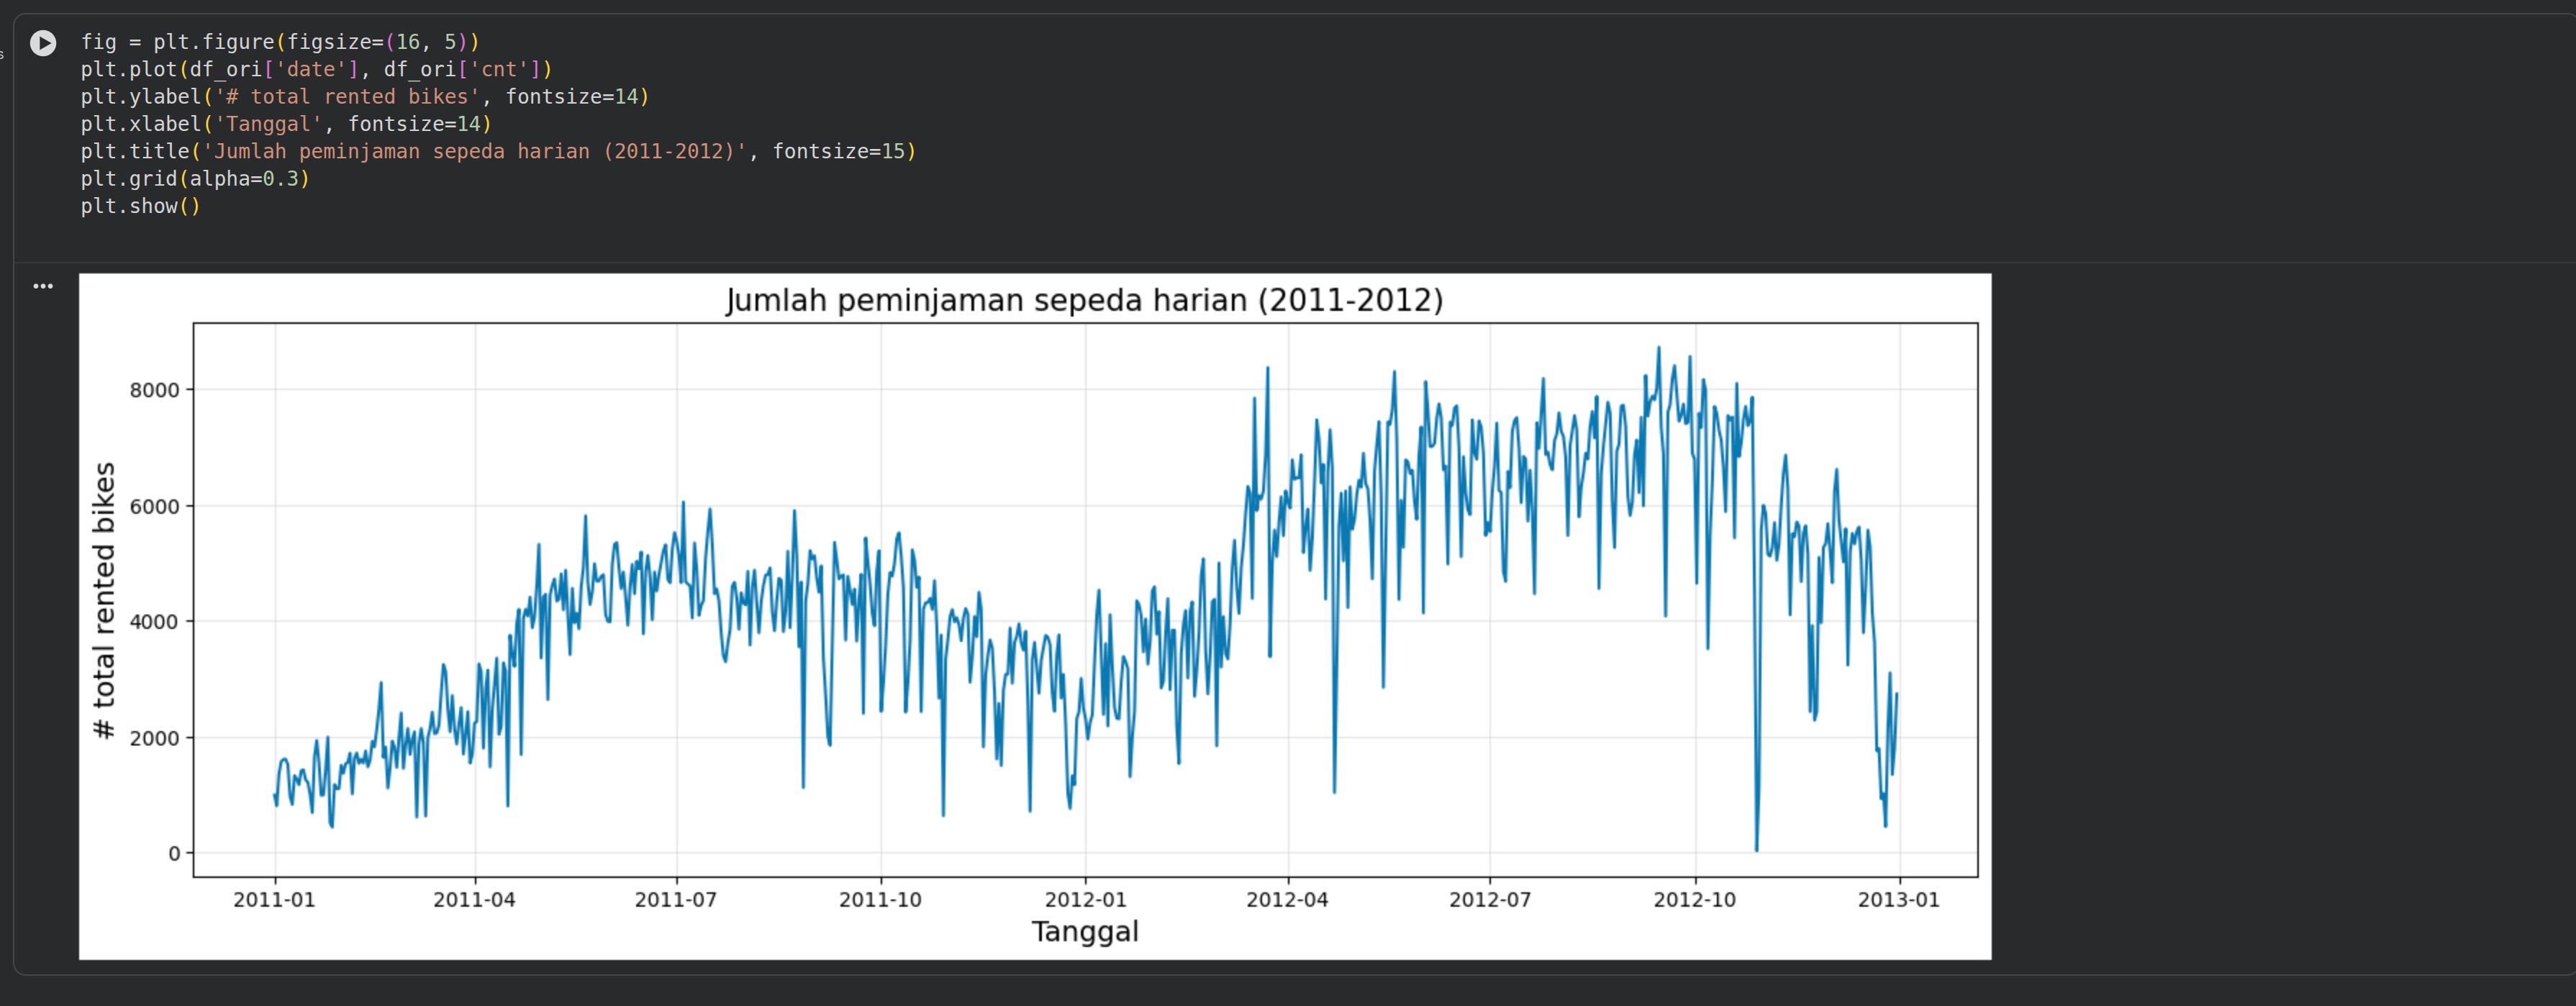
\includegraphics[width=0.98\textwidth]{images/t03-timeseries.png}}
\caption{Deret waktu jumlah peminjaman sepeda harian sepanjang 2011 sampai 2012. Terlihat pola musiman naik-turun dan tren yang menguat pada tahun kedua.}
\label{fig:ts-bike}
\end{figure}

Grafik menunjukkan dua hal. Pertama, ada pola berulang yang menandakan pengaruh musim dan hari kerja. Kedua, jumlah peminjaman pada 2012 lebih tinggi daripada 2011, jadi datanya punya tren naik. Kedua sifat ini masuk akal untuk data peminjaman sepeda dan menjelaskan mengapa model berbasis pola historis bisa bekerja cukup baik.

\subsection{Pelatihan Model dan Prediksi}
Saya melatih lima model dengan fungsi terpisah. Tiap fungsi melatih model pada data latih, memprediksi data uji, membulatkan hasil prediksi, lalu menghitung RMSE dan Pearson.

\begin{lstlisting}[style=pythonstyle,caption={Fungsi model MLP (contoh, model lain mengikuti pola yang sama).}]
def mlp(X_train, X_test, y_train, y_test):
    model = MLPRegressor(random_state=42)
    model.fit(X_train, y_train)
    y_pred = np.round(model.predict(X_test), 0)
    rmse = sqrt(mean_squared_error(y_test, y_pred))
    corr, _ = pearsonr(y_test, y_pred)
    return rmse, corr, y_pred
\end{lstlisting}

\begin{lstlisting}[style=pythonstyle,caption={Memanggil kelima model.}]
rmse_mlp, corr_mlp, y_pred_mlp = mlp(X_train, X_test, y_train, y_test)
rmse_knn, corr_knn, y_pred_knn = knn(X_train, X_test, y_train, y_test)
rmse_dt,  corr_dt,  y_pred_dt  = dt(X_train, X_test, y_train, y_test)
rmse_svm, corr_svm, y_pred_svm = svm(X_train, X_test, y_train, y_test)
rmse_rf,  corr_rf,  y_pred_rf  = rf(X_train, X_test, y_train, y_test)
\end{lstlisting}

\subsection{Visualisasi Hasil Prediksi}
Gambar berikut membandingkan nilai aktual dengan prediksi MLP pada seluruh data uji, lalu membandingkan empat model pada 100 sampel pertama agar perbedaannya lebih mudah dilihat.

\begin{lstlisting}[style=pythonstyle,caption={Visualisasi aktual vs prediksi.}]
fig = plt.figure(figsize=(16, 5))
plt.plot(y_test, label='Real data')
plt.plot(y_pred_mlp, label='MLP')
plt.xlabel('Time t', fontsize=14)
plt.ylabel('rented bikes', fontsize=14)
plt.legend(loc='upper left', fontsize=13)
plt.show()
\end{lstlisting}

\begin{figure}[H]
\centering
\customfbox{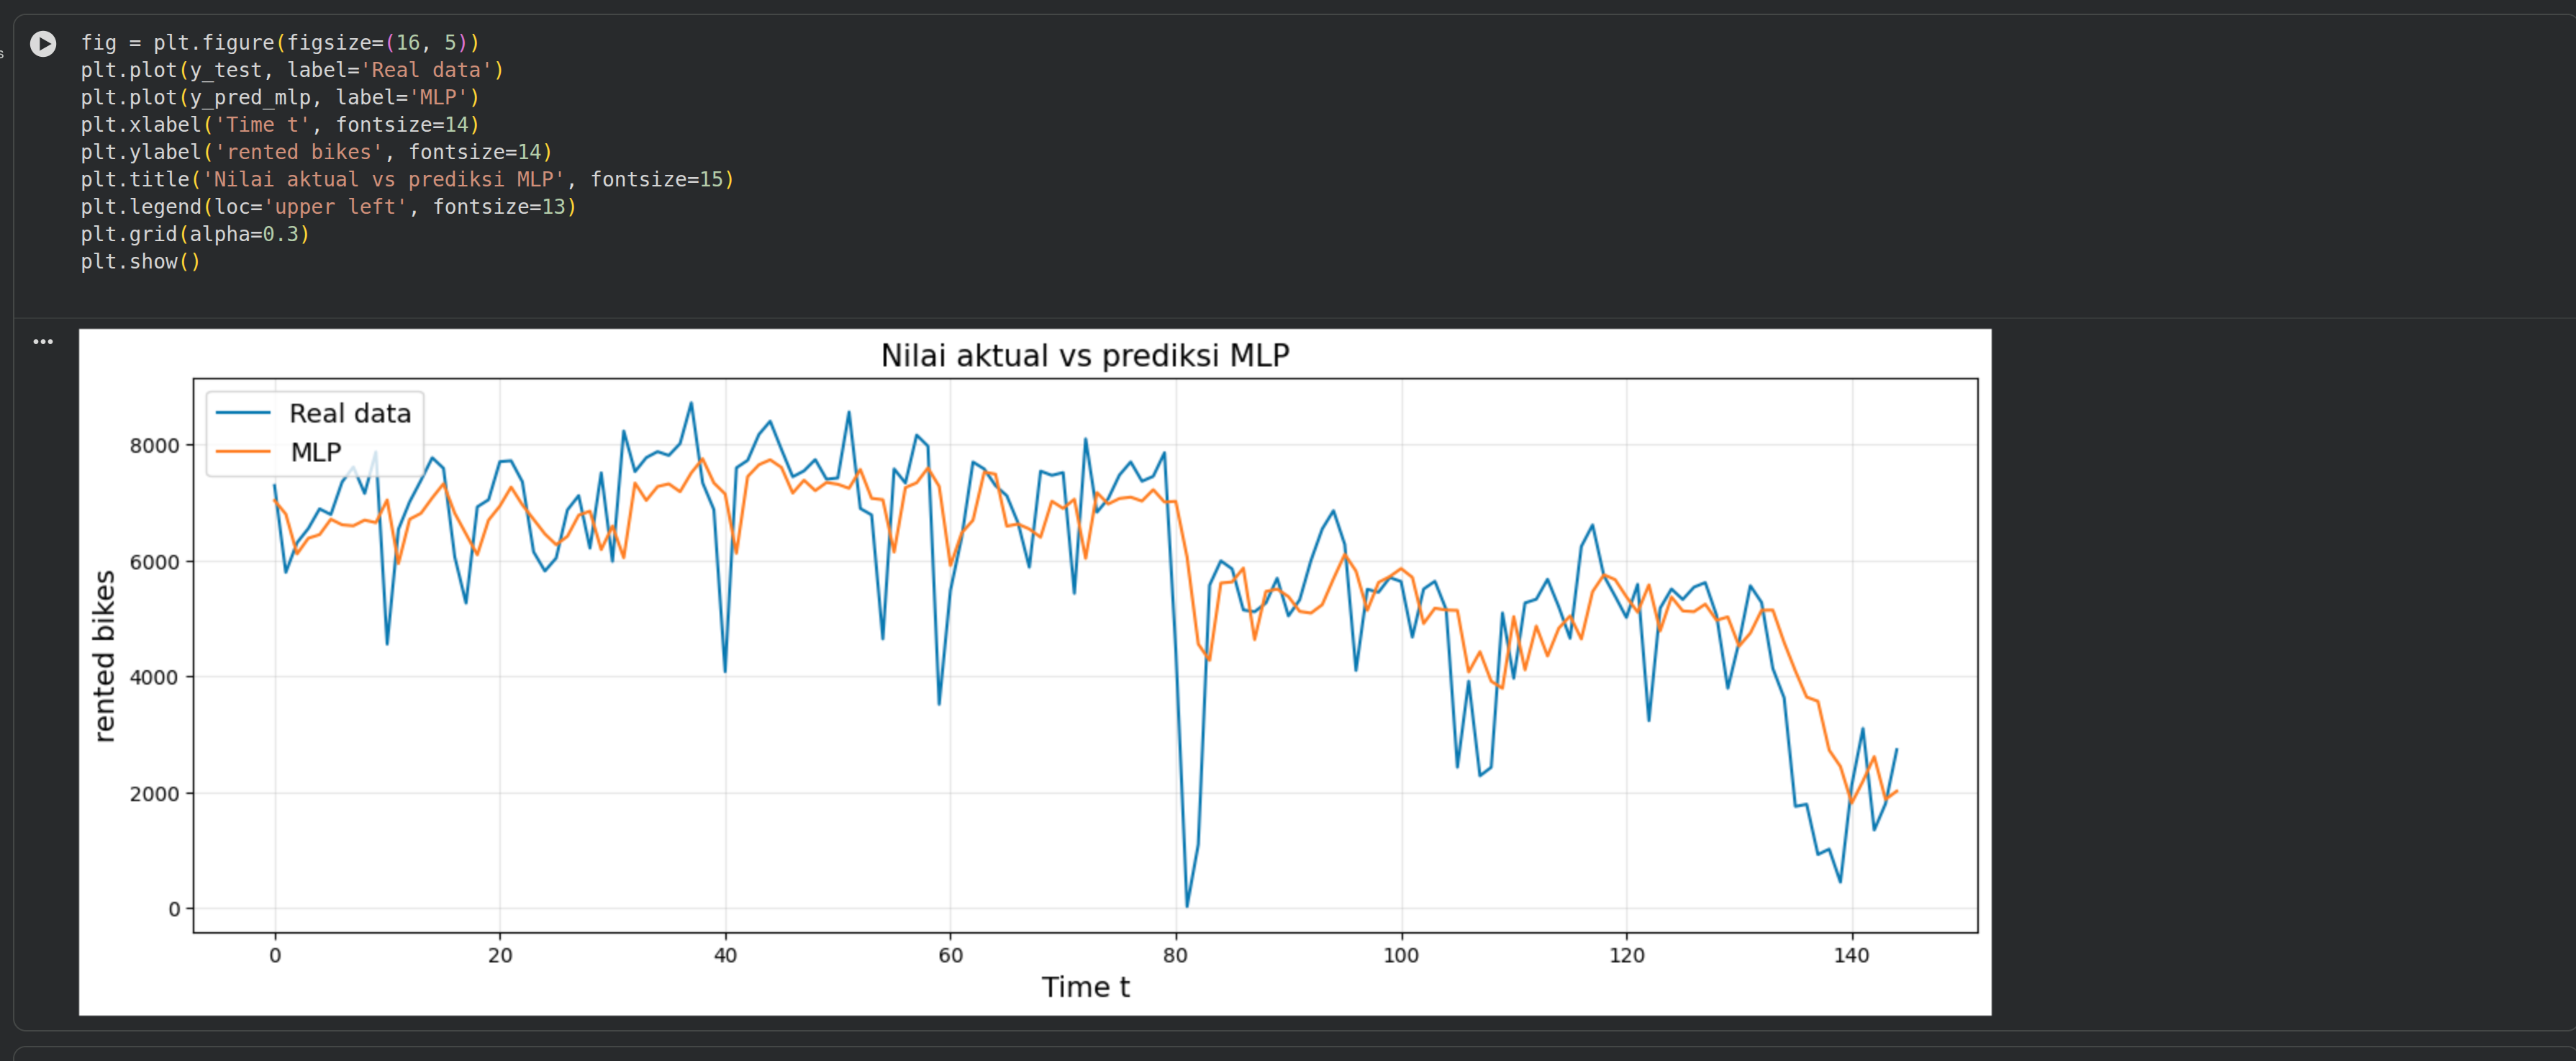
\includegraphics[width=0.98\textwidth]{images/t04-aktual-mlp.png}}
\caption{Nilai aktual (biru) dibandingkan prediksi MLP (oranye) pada data uji. Kedua garis mengikuti pola yang mirip, meski prediksi tampak lebih halus dan melewatkan sebagian puncak.}
\label{fig:aktual-mlp}
\end{figure}

\begin{figure}[H]
\centering
\customfbox{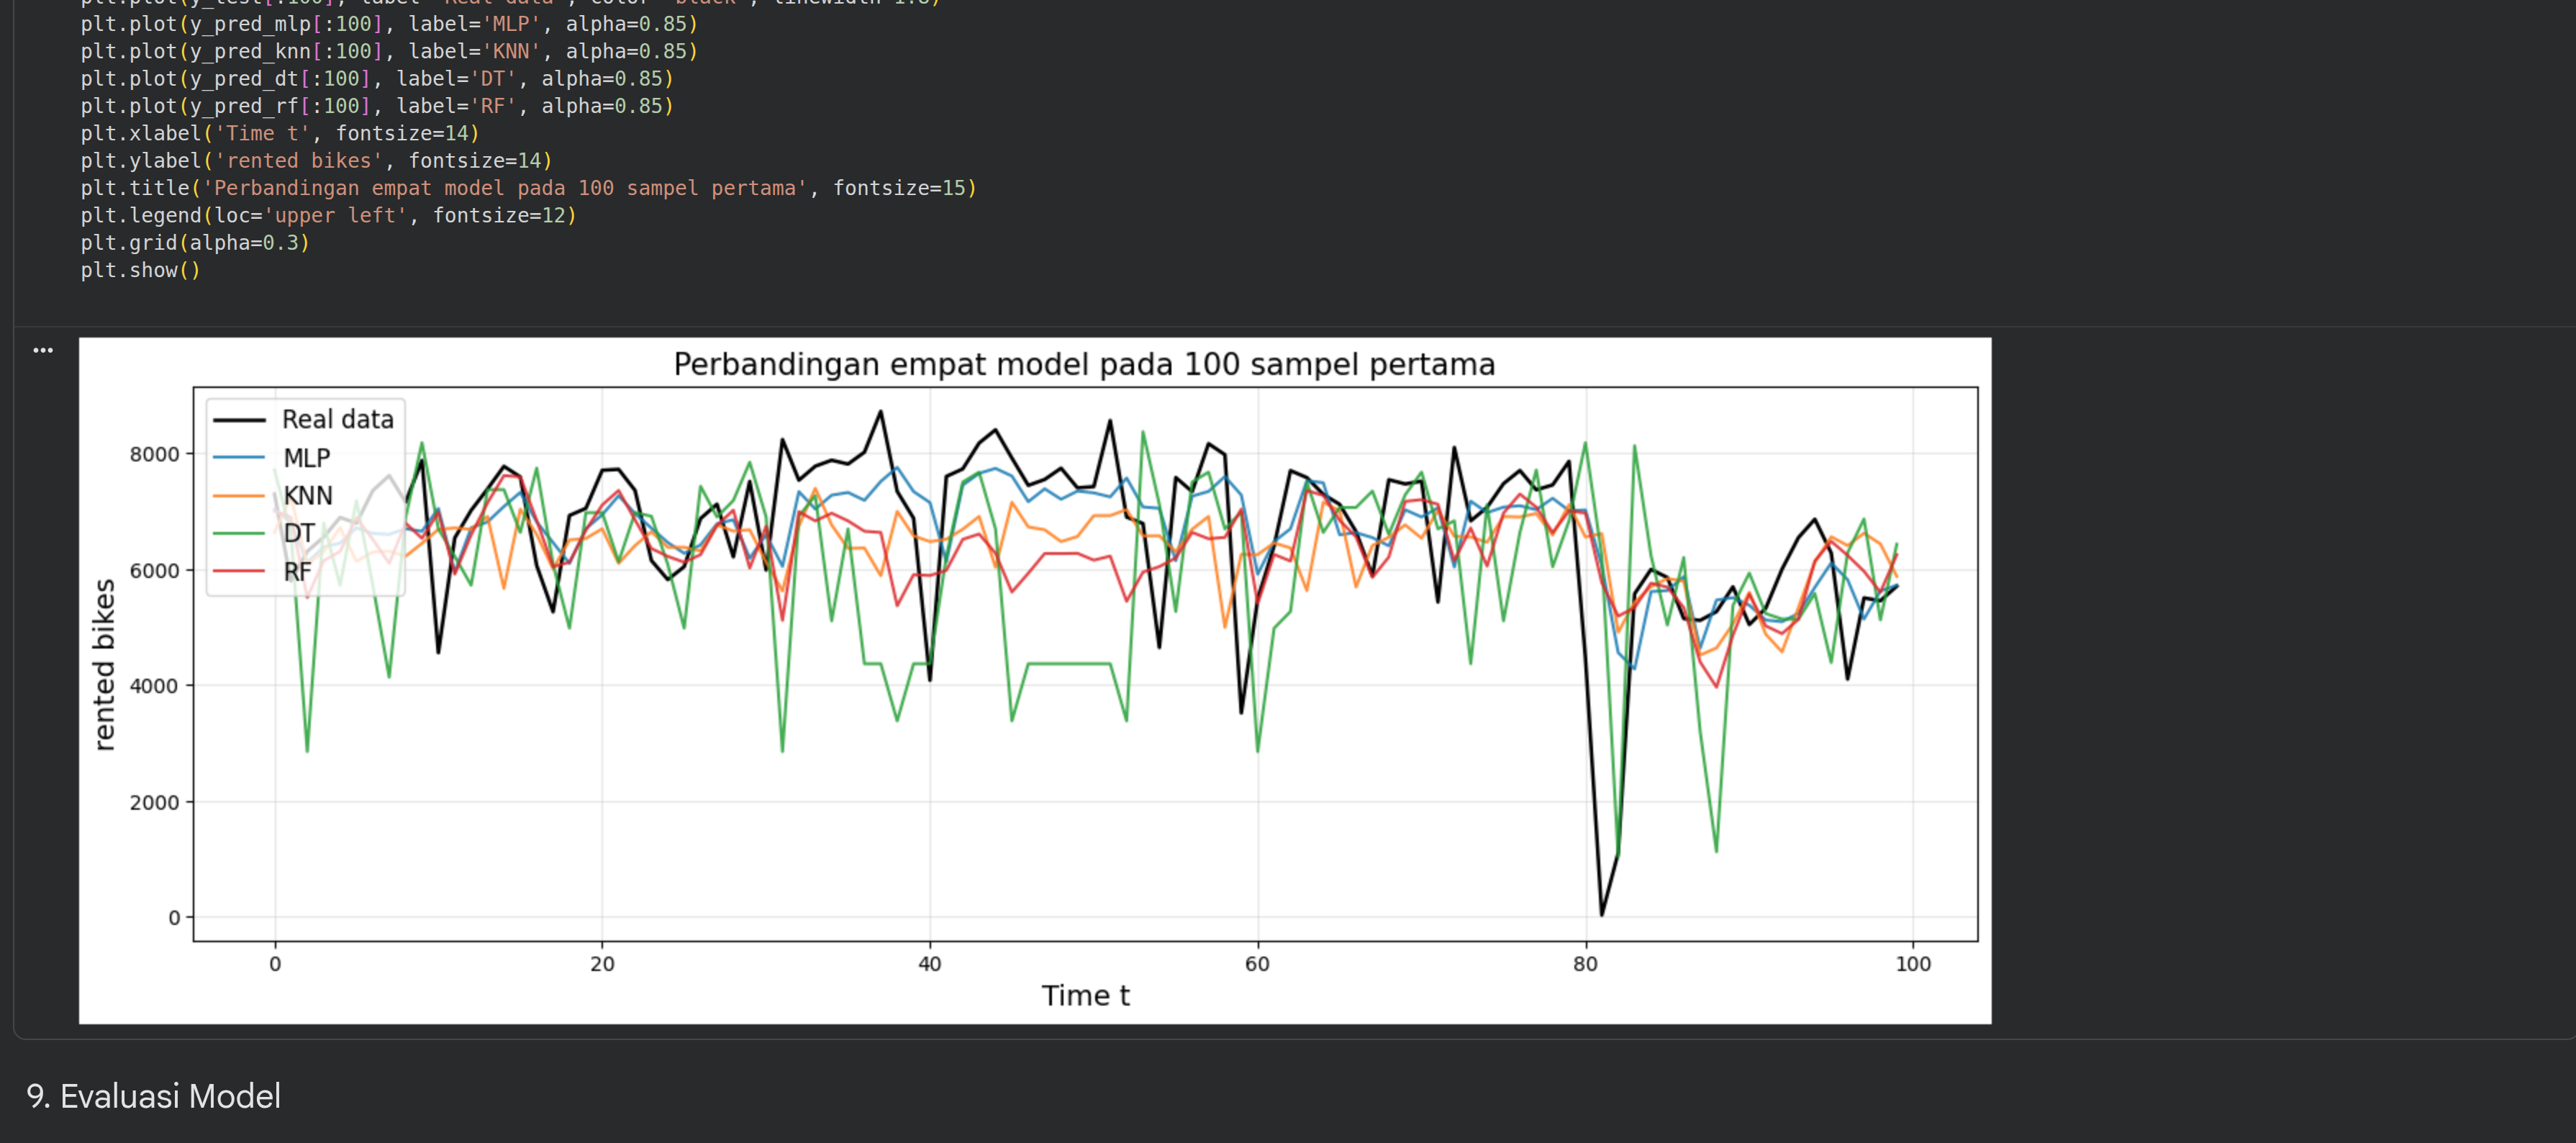
\includegraphics[width=0.98\textwidth]{images/t05-4model.png}}
\caption{Perbandingan empat model pada 100 sampel pertama. MLP paling rapat mengikuti data aktual, sedangkan Decision Tree terlihat paling jauh dari pola.}
\label{fig:semua-model}
\end{figure}

Prediksi MLP mengikuti bentuk umum data aktual, tetapi garisnya lebih mulus. Puncak peminjaman yang tinggi cenderung diprediksi lebih rendah, karena model cenderung menahan prediksi mendekati rata-rata pola yang pernah dilihatnya. Pada perbandingan empat model, Decision Tree terlihat paling jarang menyesuaikan diri dengan pola, sementara MLP dan Random Forest lebih rapat.

\subsection{Evaluasi Model}
Evaluasi memakai RMSE dan Pearson untuk kelima model.

\begin{lstlisting}[style=pythonstyle,caption={Mencetak RMSE dan Pearson tiap model.}]
for name, rmse, corr in [
    ('MLP', rmse_mlp, corr_mlp),
    ('KNN', rmse_knn, corr_knn),
    ('DT',  rmse_dt,  corr_dt),
    ('SVR', rmse_svm, corr_svm),
    ('RF',  rmse_rf,  corr_rf),
]:
    print('________________________')
    print(name)
    print('RMSE: %.3f' % rmse)
    print('Pearson correlation coefficient: %.3f' % corr)
\end{lstlisting}

\begin{figure}[H]
\centering
\customfbox{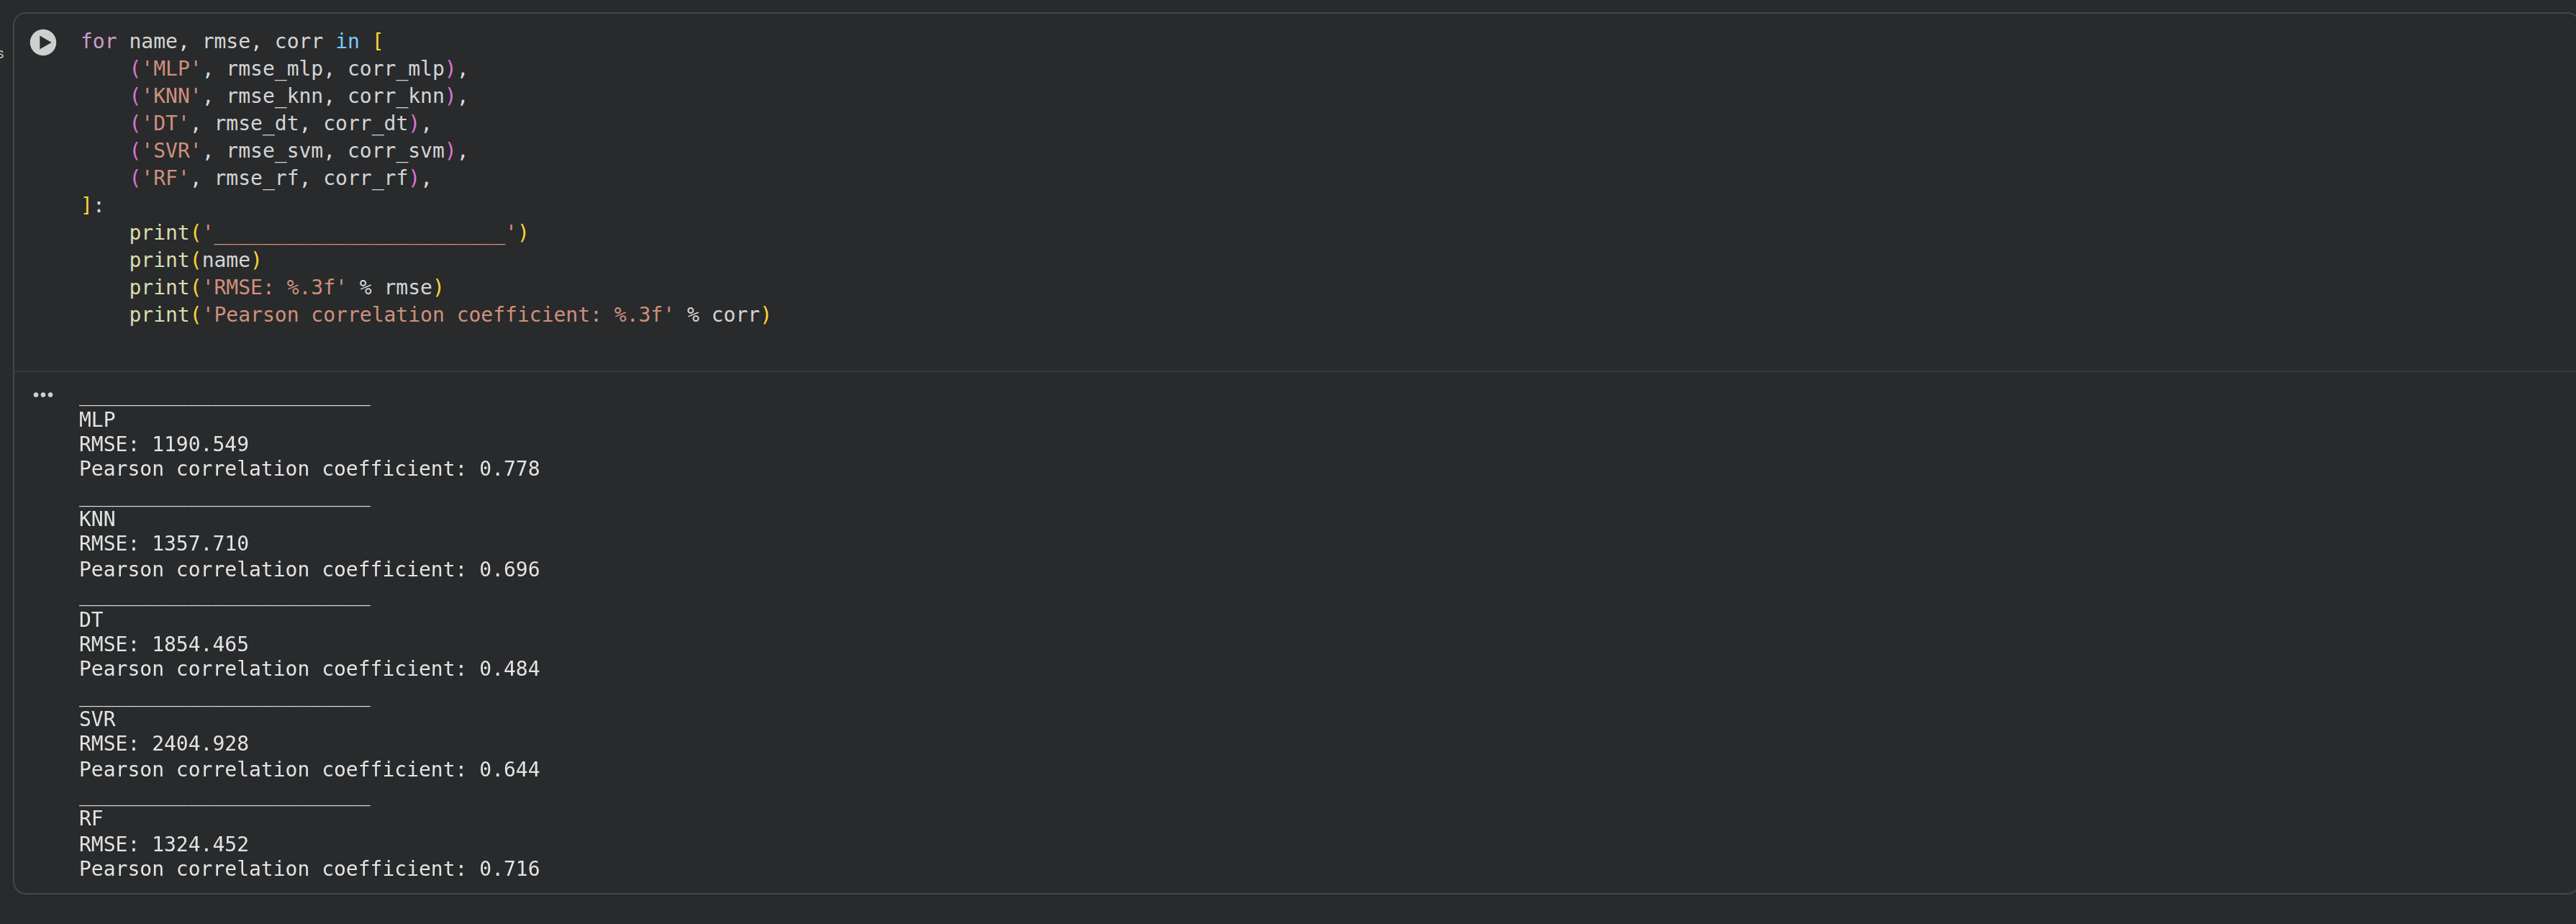
\includegraphics[width=0.6\textwidth]{images/t06-eval-bike.png}}
\caption{Hasil evaluasi kelima model pada dataset bike sharing.}
\label{fig:eval-bike}
\end{figure}

\begin{table}[H]
\centering
\small
\begin{tabular}{lcc}
\toprule
\textbf{Model} & \textbf{RMSE} & \textbf{Pearson} \\
\midrule
MLP (Neural Network) & 1190,549 & 0,778 \\
Random Forest & 1324,452 & 0,716 \\
KNN & 1357,710 & 0,696 \\
Decision Tree & 1854,465 & 0,484 \\
SVR & 2404,928 & 0,644 \\
\bottomrule
\end{tabular}
\caption{Perbandingan performa lima model pada dataset bike sharing (split 80:20, \texttt{shuffle=False}).}
\label{tab:performa-bike}
\end{table}

MLP menempati urutan pertama pada kedua metrik: RMSE terendah 1190,549 dan Pearson tertinggi 0,778. Random Forest menyusul dengan RMSE 1324,452, sedikit lebih baik daripada KNN. Decision Tree jadi model terlemah dari sisi Pearson (0,484) karena pohon tunggal mudah menyesuaikan diri berlebihan pada data latih, sehingga prediksinya kurang mulus ketika menghadapi data uji. SVR memberi RMSE tertinggi 2404,928; nilai bawaannya bekerja pada skala fitur asli, sedangkan fitur di sini tidak dinormalisasi, sehingga hasilnya kurang optimal. Temuan ini sesuai dengan catatan pada bagian dasar teori bahwa SVR sebaiknya dipakai bersama normalisasi.

\subsection{Perbandingan dengan Baseline Naif}
Untuk menilai apakah model benar-benar belajar, saya membandingkan hasilnya dengan \textit{baseline} sederhana yang memprediksi nilai besok sama dengan nilai hari terakhir pada jendela. Baseline ini hanya mengulang angka terakhir tanpa belajar pola.

\begin{lstlisting}[style=pythonstyle,caption={Menghitung RMSE baseline naif.}]
last_value = X[:, -1]
rmse_naive = sqrt(mean_squared_error(y_test, last_value[-len(y_test):]))
print('naive RMSE: %.3f' % rmse_naive)
\end{lstlisting}

\begin{figure}[H]
\centering
\customfbox{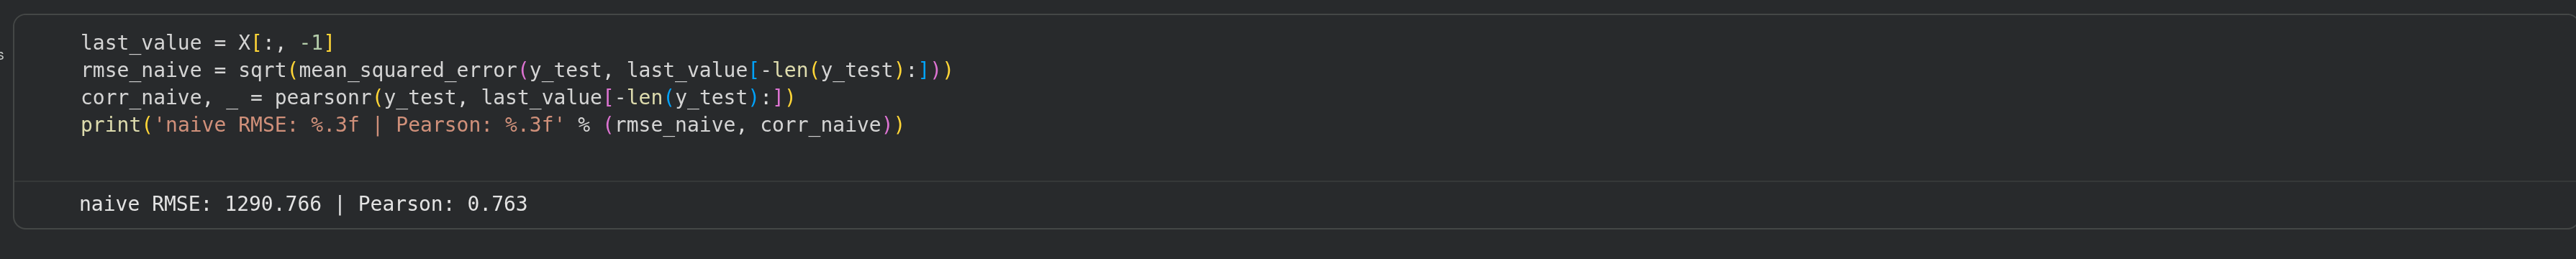
\includegraphics[width=0.9\textwidth]{images/t07-naive.png}}
\caption{Output perhitungan RMSE baseline naif pada notebook.}
\label{fig:naive}
\end{figure}

Baseline naif menghasilkan RMSE 1290,766. MLP (1190,549) dan Random Forest (1324,452) berada di sekitar angka itu. Artinya untuk data peminjaman sepeda yang berfluktuasi harian, sebagian besar nilai prediksi yang wajar bisa didapat hanya dengan mengulang nilai terakhir. Keunggulan MLP di sini nyata, tetapi tidak besar, dan patut dibaca dengan hati-hati.

\clearpage

\section{Tugas dan Analisis: Forecasting Harga Saham Tesla}
Sesuai Modul 5.5, saya mengerjakan tugas dengan dataset \textit{Tesla Stock Data from 2010 to 2020} \cite{kaggle-tesla}. Dataset ini memuat harga saham Tesla harian. Karena Kaggle memerlukan unduhan manual, saya memakai mirror GitHub \cite{tesla-mirror} yang memuat isi yang sama.

\subsection{Deskripsi Dataset dan Atribut}
Dataset berisi 2.657 baris dengan delapan kolom, mencakup rentang 29 Juni 2010 sampai 15 Januari 2021.

\begin{lstlisting}[style=pythonstyle,caption={Memuat dan memeriksa dataset Tesla.}]
ts = pd.read_csv('https://raw.githubusercontent.com/0xpranjal/Stock-Prediction-using-different-models/main/TSLA.CSV')
print('shape:', ts.shape)
print('rentang:', ts['Date'].iloc[0], '->', ts['Date'].iloc[-1])
ts.head()
\end{lstlisting}

\begin{figure}[H]
\centering
\customfbox{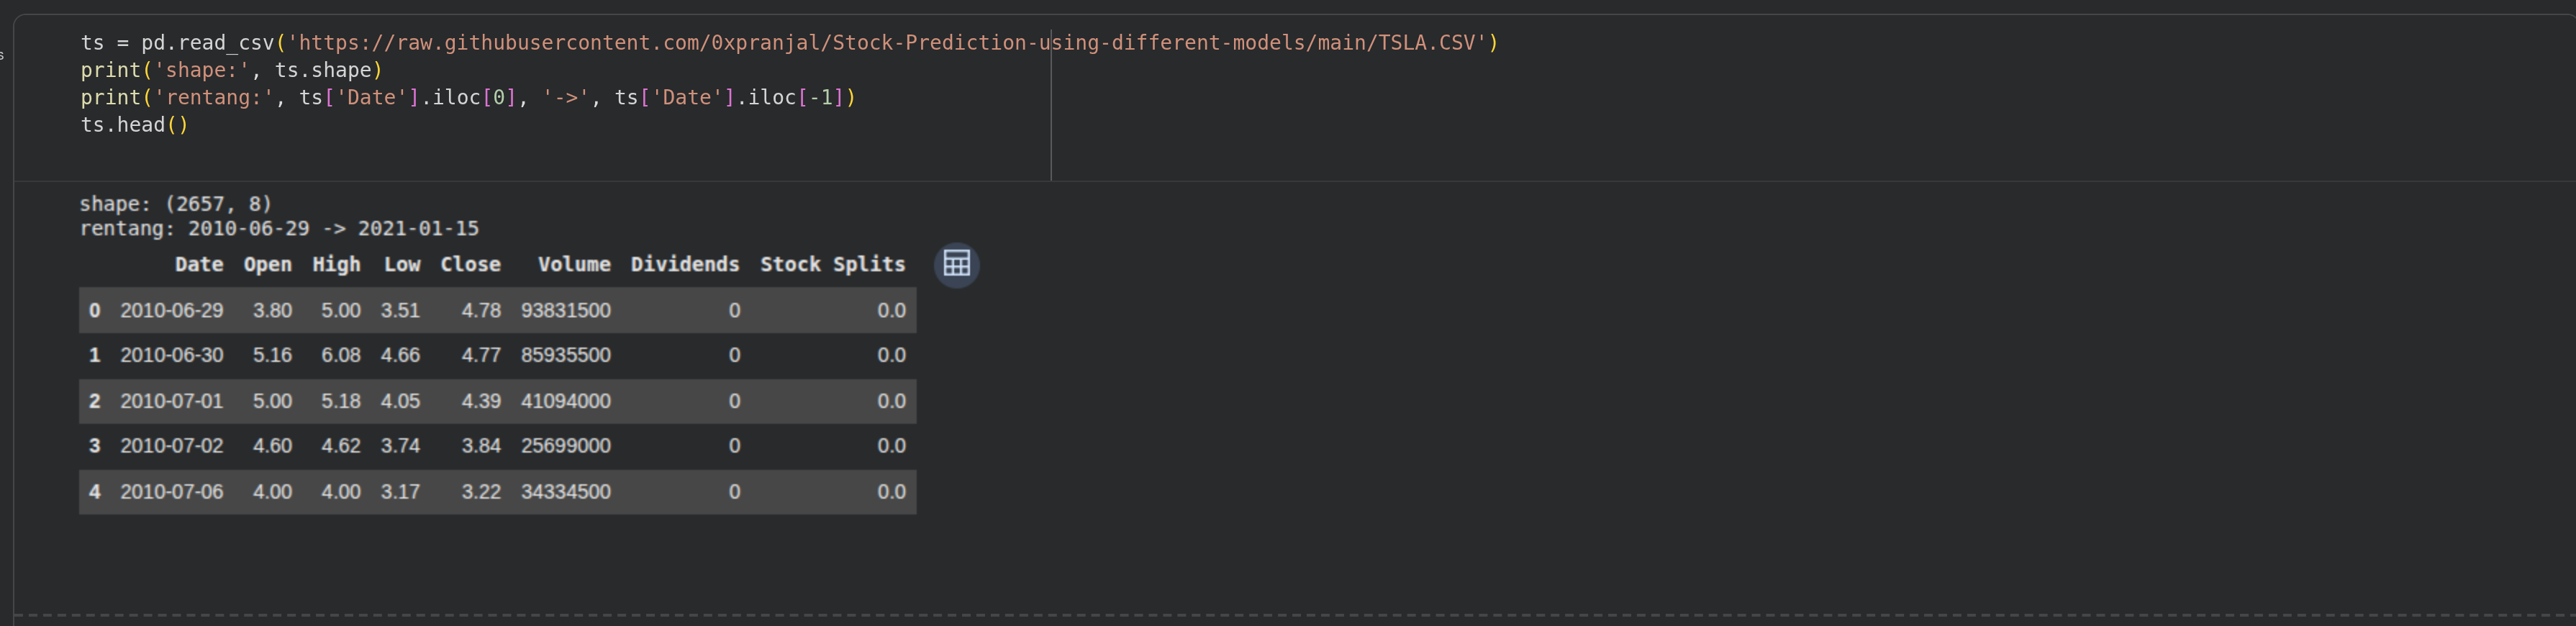
\includegraphics[width=0.9\textwidth]{images/t15-tesla-head.png}}
\caption{Lima baris pertama dataset Tesla: kolom \texttt{Date}, \texttt{Open}, \texttt{High}, \texttt{Low}, \texttt{Close}, \texttt{Volume}, \texttt{Dividends}, dan \texttt{Stock Splits}.}
\label{fig:tesla-head}
\end{figure}

\begin{table}[H]
\centering
\small
\begin{tabular}{|p{2.6cm}|p{11.2cm}|}
\hline
\textbf{Atribut} & \textbf{Penjelasan} \\
\hline
\texttt{Date} & Tanggal perdagangan. \\
\texttt{Open} & Harga pembukaan pada hari tersebut. \\
\texttt{High} & Harga tertinggi hari itu. \\
\texttt{Low} & Harga terendah hari itu. \\
\texttt{Close} & Harga penutupan, menjadi target prediksi. \\
\texttt{Volume} & Jumlah saham yang diperdagangkan. \\
\texttt{Dividends} & Pembayaran dividen, seluruhnya nol pada dataset ini. \\
\texttt{Stock Splits} & Rasio pemecahan saham, seluruhnya nol pada dataset ini. \\
\hline
\end{tabular}
\caption{Deskripsi atribut dataset Tesla.}
\label{tab:tesla-attributes}
\end{table}

Harga penutupan (\texttt{Close}) bergerak dari 3,16 sampai 880,02 dolar dengan rata-rata 63,67 dan standar deviasi 104,06. Rentang yang lebar ini menandakan kenaikan harga yang besar selama sepuluh tahun, dan pola seperti ini menjadi kunci pada pembahasan hasil nanti.

\begin{figure}[H]
\centering
\customfbox{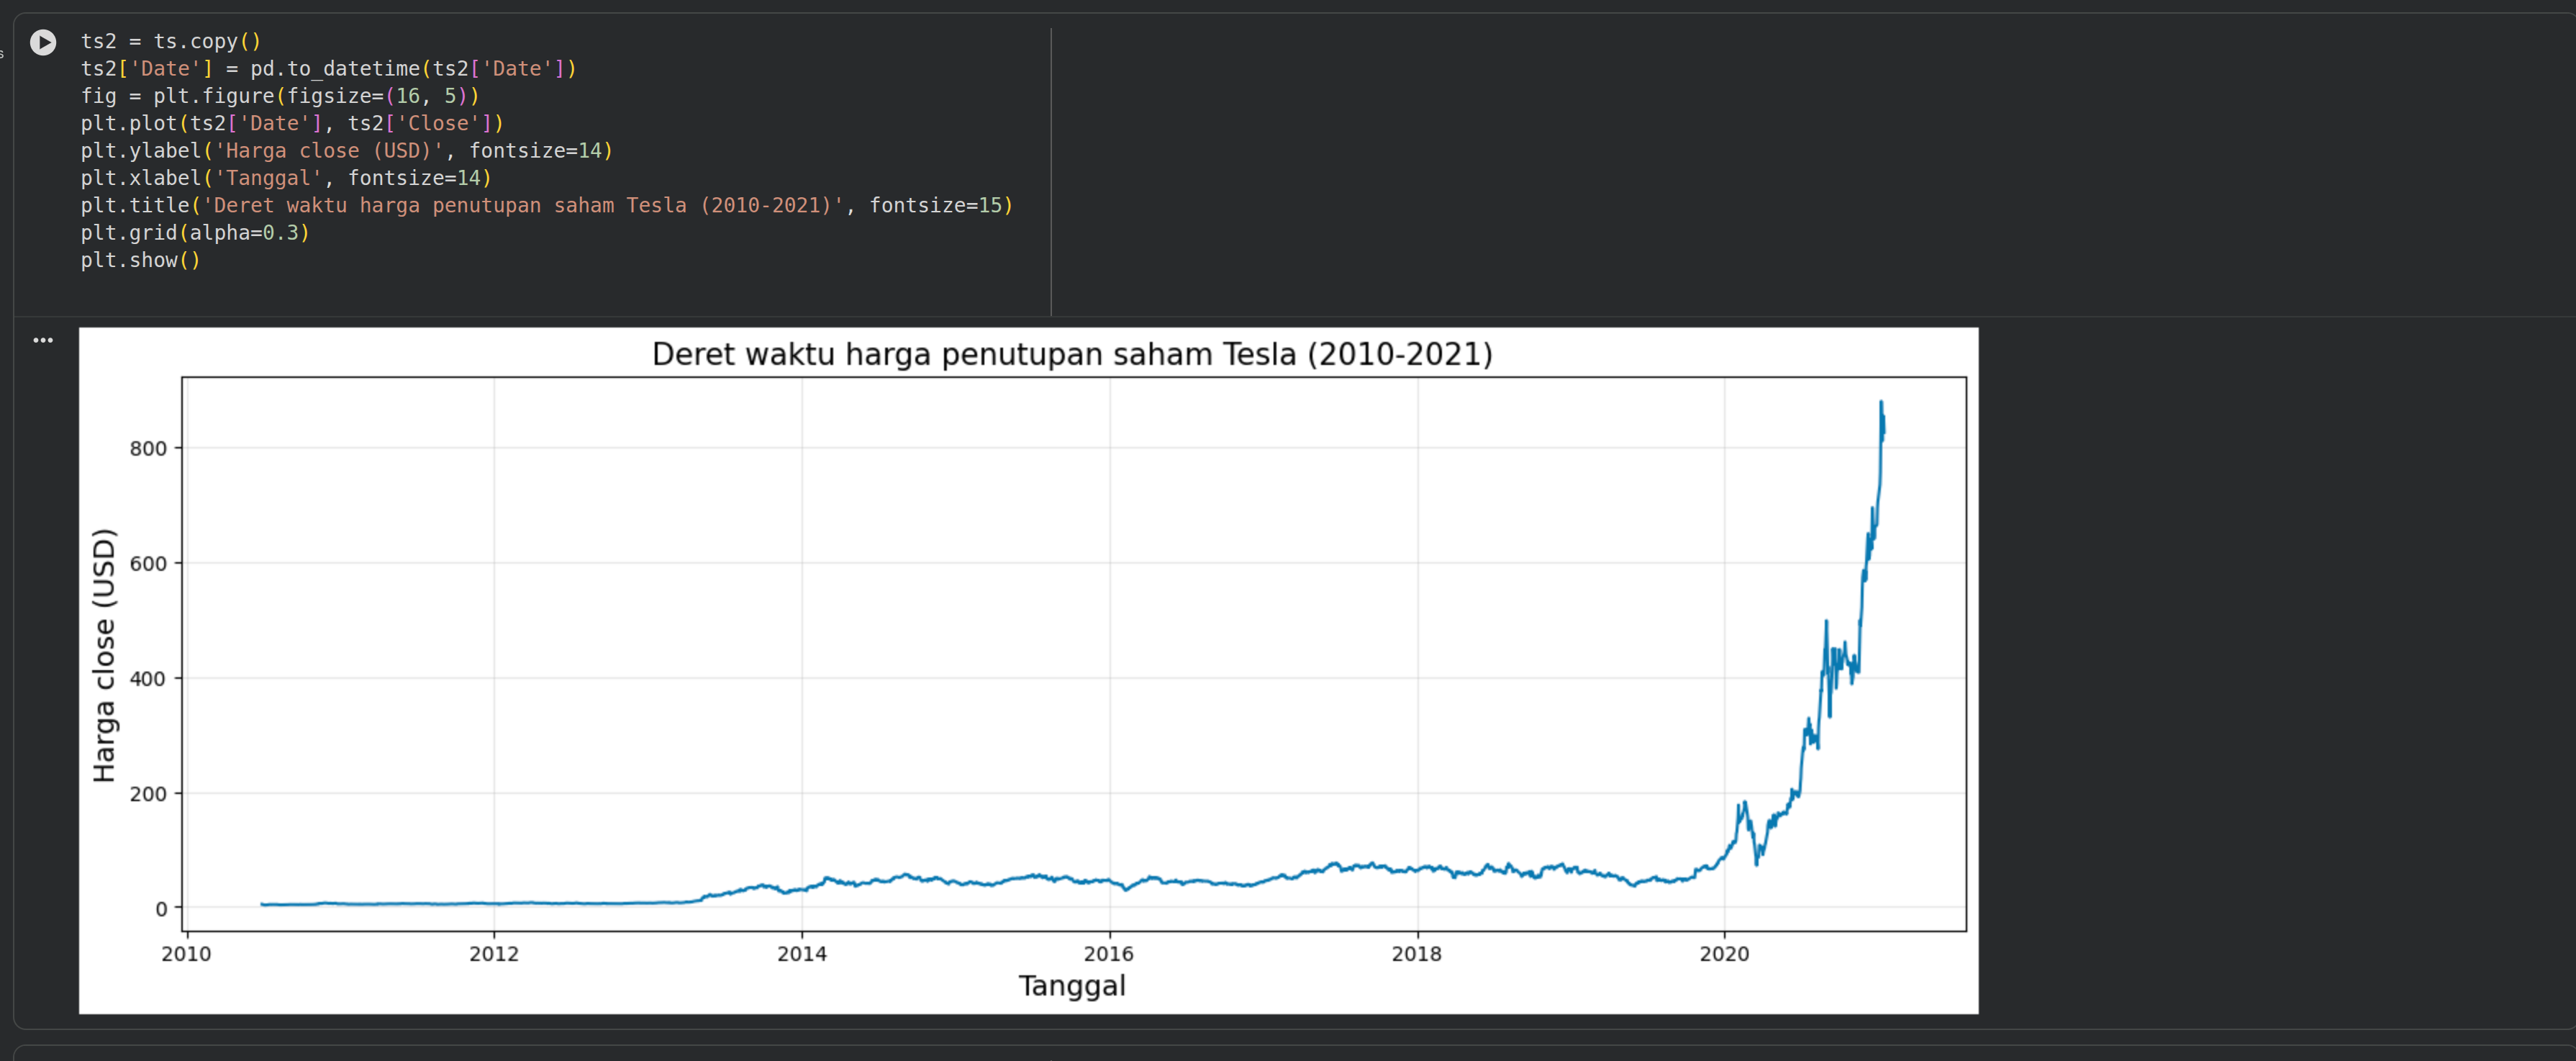
\includegraphics[width=0.98\textwidth]{images/t08-tesla-ts.png}}
\caption{Deret waktu harga penutupan saham Tesla 2010 sampai 2021. Harga relatif datar pada tahun-tahun awal, lalu naik tajam menjelang akhir periode.}
\label{fig:ts-tesla}
\end{figure}

\subsection{Skenario A: Prediksi dari Close 7 Hari Sebelumnya}
Tugas pertama meminta prediksi \texttt{Close} dua hari ke depan memakai \texttt{Close} tujuh hari sebelumnya. Karena targetnya dua langkah ke depan, \texttt{n\_steps\_out} diisi 2.

\begin{lstlisting}[style=pythonstyle,caption={Skenario A: masukan hanya Close.}]
df_A = ts[['Close', 'Close']]
seq_A = df_A.astype(float).values
XA, yA = split_sequences(seq_A, 7, 2)
XA = XA.reshape((XA.shape[0], XA.shape[1] * XA.shape[2]))
XA_tr, XA_te, yA_tr, yA_te = train_test_split(
    XA, yA, test_size=0.2, random_state=42, shuffle=False)
XA_tr = stats_features(XA_tr)
XA_te = stats_features(XA_te)

resA = {}
resA['MLP'] = mlp(XA_tr, XA_te, yA_tr, yA_te)
resA['KNN'] = knn(XA_tr, XA_te, yA_tr, yA_te)
resA['DT']  = dt(XA_tr, XA_te, yA_tr, yA_te)
resA['SVR'] = svm(XA_tr, XA_te, yA_tr, yA_te)
resA['RF']  = rf(XA_tr, XA_te, yA_tr, yA_te)
\end{lstlisting}

\subsection{Skenario B: Prediksi dari Close dan Open 7 Hari Sebelumnya}
Tugas kedua menambah \texttt{Open} sebagai fitur. Karena ada dua kolom masukan, jendela berisi 14 nilai mentah sebelum fitur statistik ditambahkan, sehingga totalnya menjadi 22 fitur.

\begin{lstlisting}[style=pythonstyle,caption={Skenario B: masukan Close dan Open.}]
df_B = ts[['Close', 'Open', 'Close']]
seq_B = df_B.astype(float).values
XB, yB = split_sequences(seq_B, 7, 2)
XB = XB.reshape((XB.shape[0], XB.shape[1] * XB.shape[2]))
XB_tr, XB_te, yB_tr, yB_te = train_test_split(
    XB, yB, test_size=0.2, random_state=42, shuffle=False)
XB_tr = stats_features(XB_tr)
XB_te = stats_features(XB_te)

resB = {}
resB['MLP'] = mlp(XB_tr, XB_te, yB_tr, yB_te)
resB['KNN'] = knn(XB_tr, XB_te, yB_tr, yB_te)
resB['DT']  = dt(XB_tr, XB_te, yB_tr, yB_te)
resB['SVR'] = svm(XB_tr, XB_te, yB_tr, yB_te)
resB['RF']  = rf(XB_tr, XB_te, yB_tr, yB_te)
\end{lstlisting}

\begin{figure}[H]
\centering
\customfbox{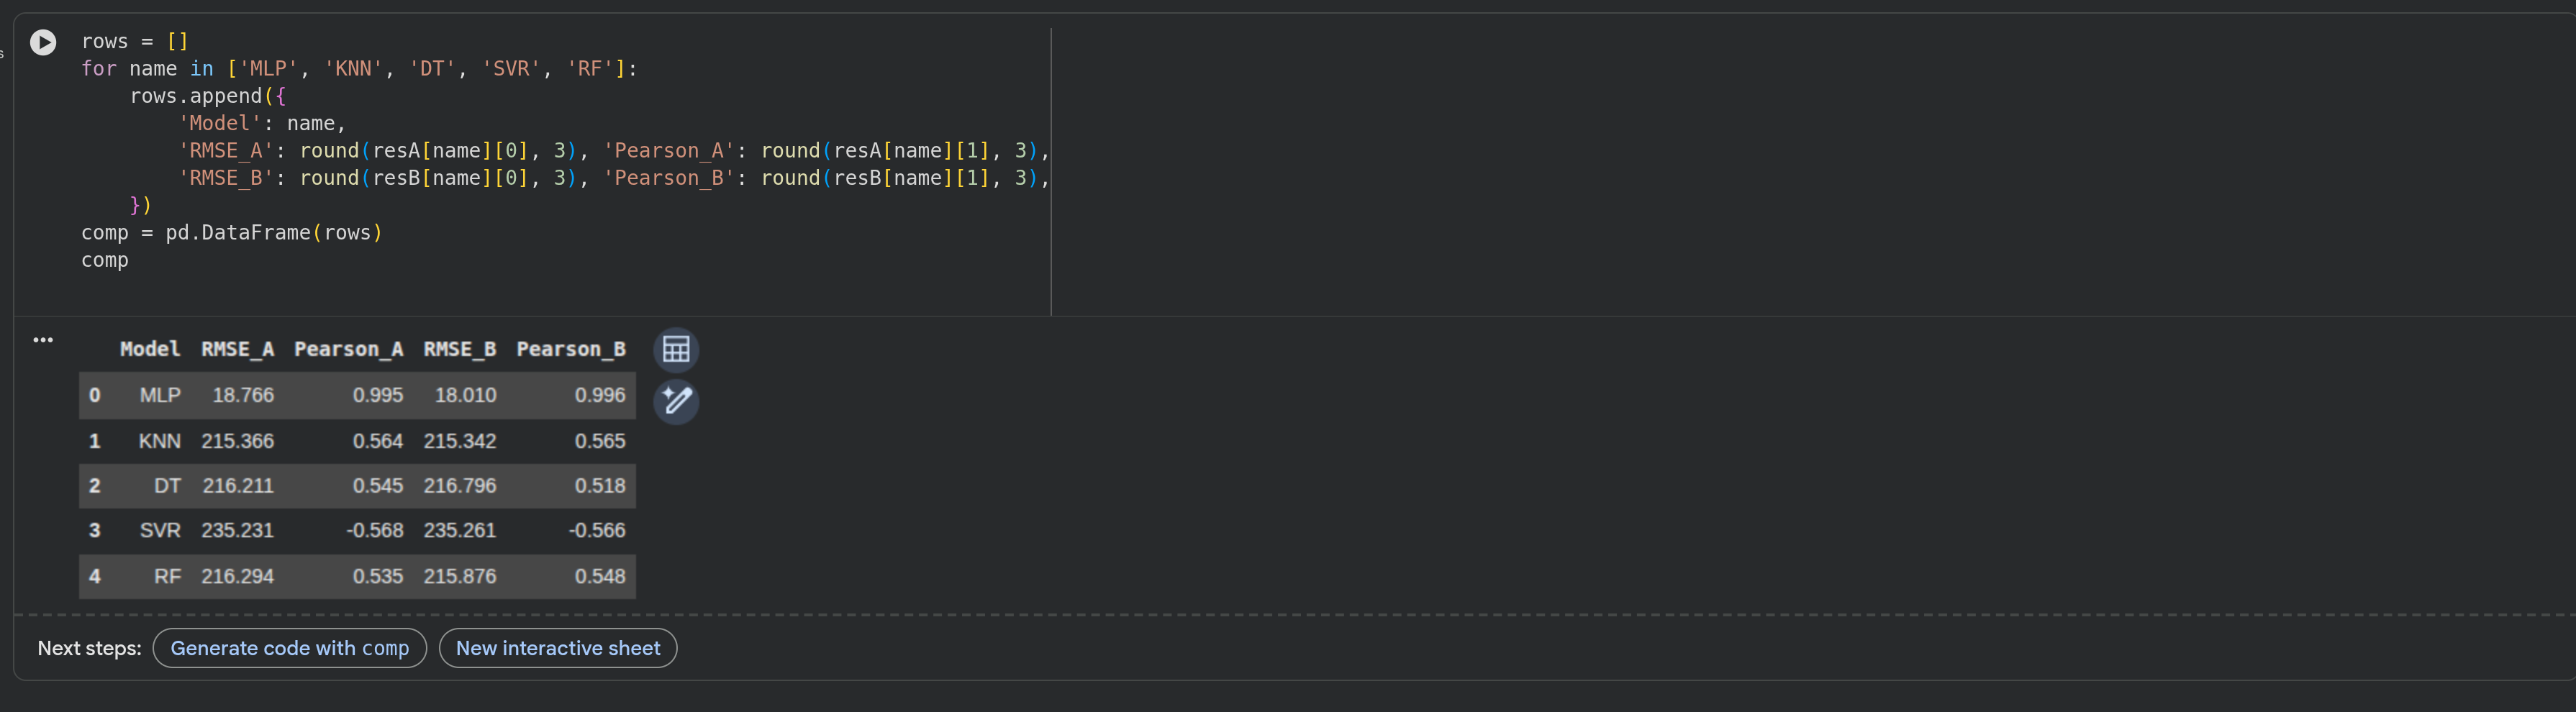
\includegraphics[width=0.85\textwidth]{images/t09-tesla-compare.png}}
\caption{Hasil evaluasi kelima model pada kedua skenario Tesla (tabel perbandingan dari Colab).}
\label{fig:eval-tesla}
\end{figure}

\begin{table}[H]
\centering
\small
\begin{tabular}{lcccc}
\toprule
 & \multicolumn{2}{c}{\textbf{Skenario A (Close)}} & \multicolumn{2}{c}{\textbf{Skenario B (Close + Open)}} \\
\cmidrule(lr){2-3} \cmidrule(lr){4-5}
\textbf{Model} & \textbf{RMSE} & \textbf{Pearson} & \textbf{RMSE} & \textbf{Pearson} \\
\midrule
MLP (Neural Network) & 18,766 & 0,995 & 18,010 & 0,996 \\
KNN & 215,366 & 0,564 & 215,342 & 0,565 \\
Random Forest & 216,294 & 0,535 & 215,876 & 0,548 \\
Decision Tree & 216,211 & 0,545 & 216,796 & 0,518 \\
SVR & 235,231 & $-0,568$ & 235,261 & $-0,566$ \\
\bottomrule
\end{tabular}
\caption{Perbandingan performa lima model pada dua skenario tugas Tesla (split 80:20, \texttt{shuffle=False}).}
\label{tab:performa-tesla}
\end{table}

\subsection{Analisis: Mengapa MLP Unggul di Sini}
Selisih antara MLP dan empat model lain pada dataset Tesla terlalu besar untuk diabaikan. RMSE MLP 18,766 sementara KNN, Random Forest, dan Decision Tree semuanya di kisaran 215, sekitar sebelas kali lebih besar. Saya menelusuri penyebabnya dengan memeriksa rentang nilai data latih dan data uji.

\begin{lstlisting}[style=pythonstyle,caption={Memeriksa rentang target latih dan uji.}]
print('y_train: min %.2f max %.2f' % (yB_tr.min(), yB_tr.max()))
print('y_test : min %.2f max %.2f' % (yB_te.min(), yB_te.max()))
persen = 100 * np.mean(yB_te > yB_tr.max())
print('persen nilai uji di atas max latih: %.1f%%' % persen)
\end{lstlisting}

\begin{figure}[H]
\centering
\customfbox{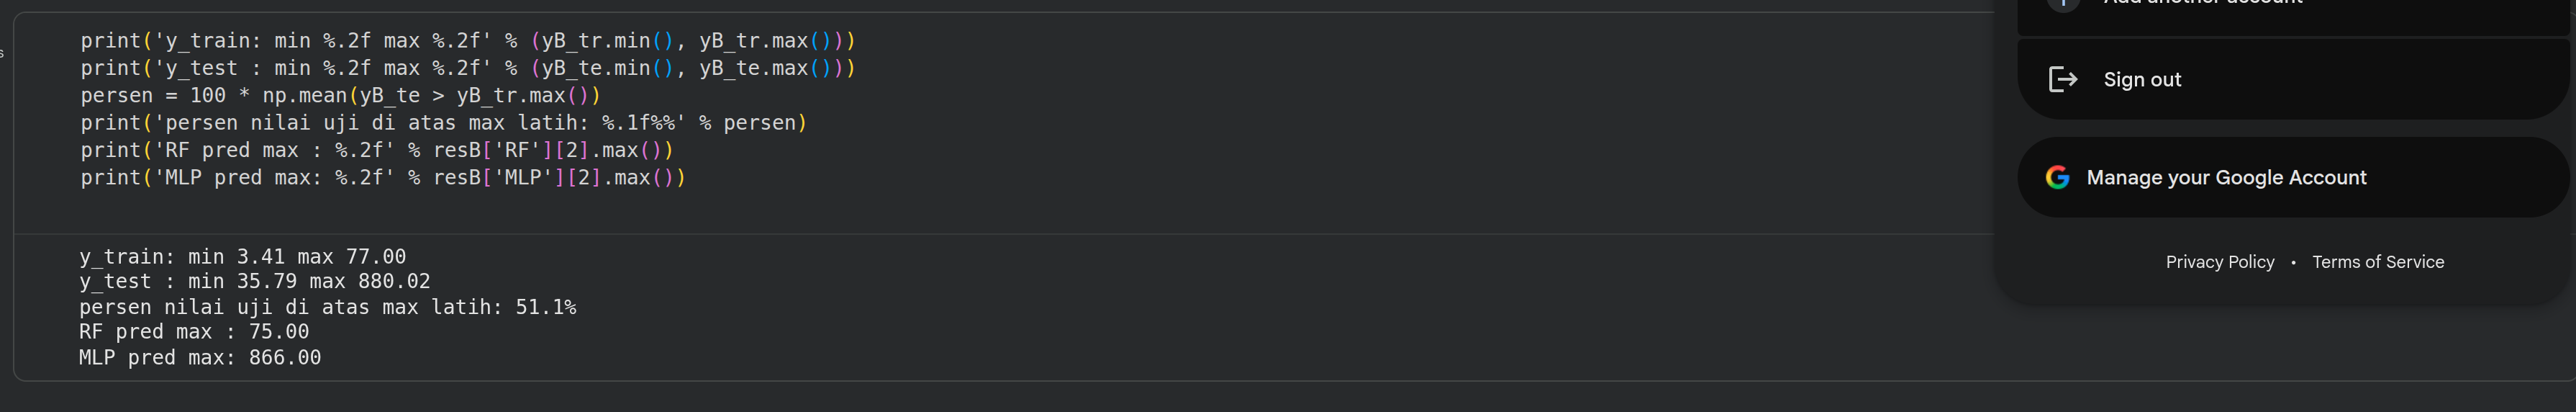
\includegraphics[width=0.9\textwidth]{images/t11-ekstrapolasi.png}}
\caption{Output pemeriksaan rentang data latih dan uji pada notebook Colab.}
\label{fig:ekstrapolasi}
\end{figure}

Hasilnya, target data latih hanya mencakup harga 3,41 sampai 77,00 dolar, sedangkan data uji mencakup 35,79 sampai 880,02 dolar. Sebanyak 51,1\% nilai uji berada di atas harga tertinggi yang pernah dilihat model saat latihan. Ini terjadi karena pembagian datanya kronologis: 80\% awal berisi periode harga murah (2010 sampai sekitar 2019), dan 20\% akhir berisi lonjakan harga Tesla (2020 sampai awal 2021).

Sifat ini membedakan model. Decision Tree, Random Forest, dan KNN hanya bisa memprediksi di dalam rentang nilai yang pernah mereka lihat, karena prediksinya berasal dari rata-rata target pada data latih. Pohon tidak bisa menghasilkan nilai di luar kotak nilai yang dikenalinya. Pemeriksaan langsung menunjukkan Random Forest memprediksi maksimum 75,00 dolar, sementara MLP bisa mencapai 866,00 dolar, mendekati harga aktual 880,02. MLP bisa melakukannya karena jaringan saraf memetakan masukan lewat fungsi kontinu yang bisa menghasilkan nilai di luar rentang data latih. Karena itu di sini MLP unggul terutama karena ia satu-satunya model yang mampu mengikuti tren naik yang belum pernah dilihatnya.

SVR memberi korelasi negatif ($-0,568$). Ini terjadi karena SVR dengan parameter bawaan cenderung menghasilkan prediksi yang hampir rata, sehingga ketika harga aktual naik tajam, arah hubungannya berbalik. Tanpa normalisasi dan penyetelan parameter, SVR tidak cocok untuk data dengan rentang harga sebesar ini.

Perlu juga saya bandingkan dengan baseline naif yang memakai harga penutupan terakhir pada jendela. Baseline ini menghasilkan RMSE 17,278 dan Pearson 0,996, sedikit lebih baik daripada MLP. Artinya pada data ini, sebagian besar akurasi berasal dari sifat harga saham yang bergerak mulus dari hari ke hari, bukan dari kemampuan model menangkap pola rumit. Prediksi dua hari ke depan dengan tujuh hari riwayat praktis mirip dengan mengulang harga terakhir. Angka RMSE di bawah 20 dolar memang terlihat bagus, tetapi perlu dibaca bersama fakta bahwa rentang harga pada data uji mencapai 880 dolar.

\begin{figure}[H]
\centering
\customfbox{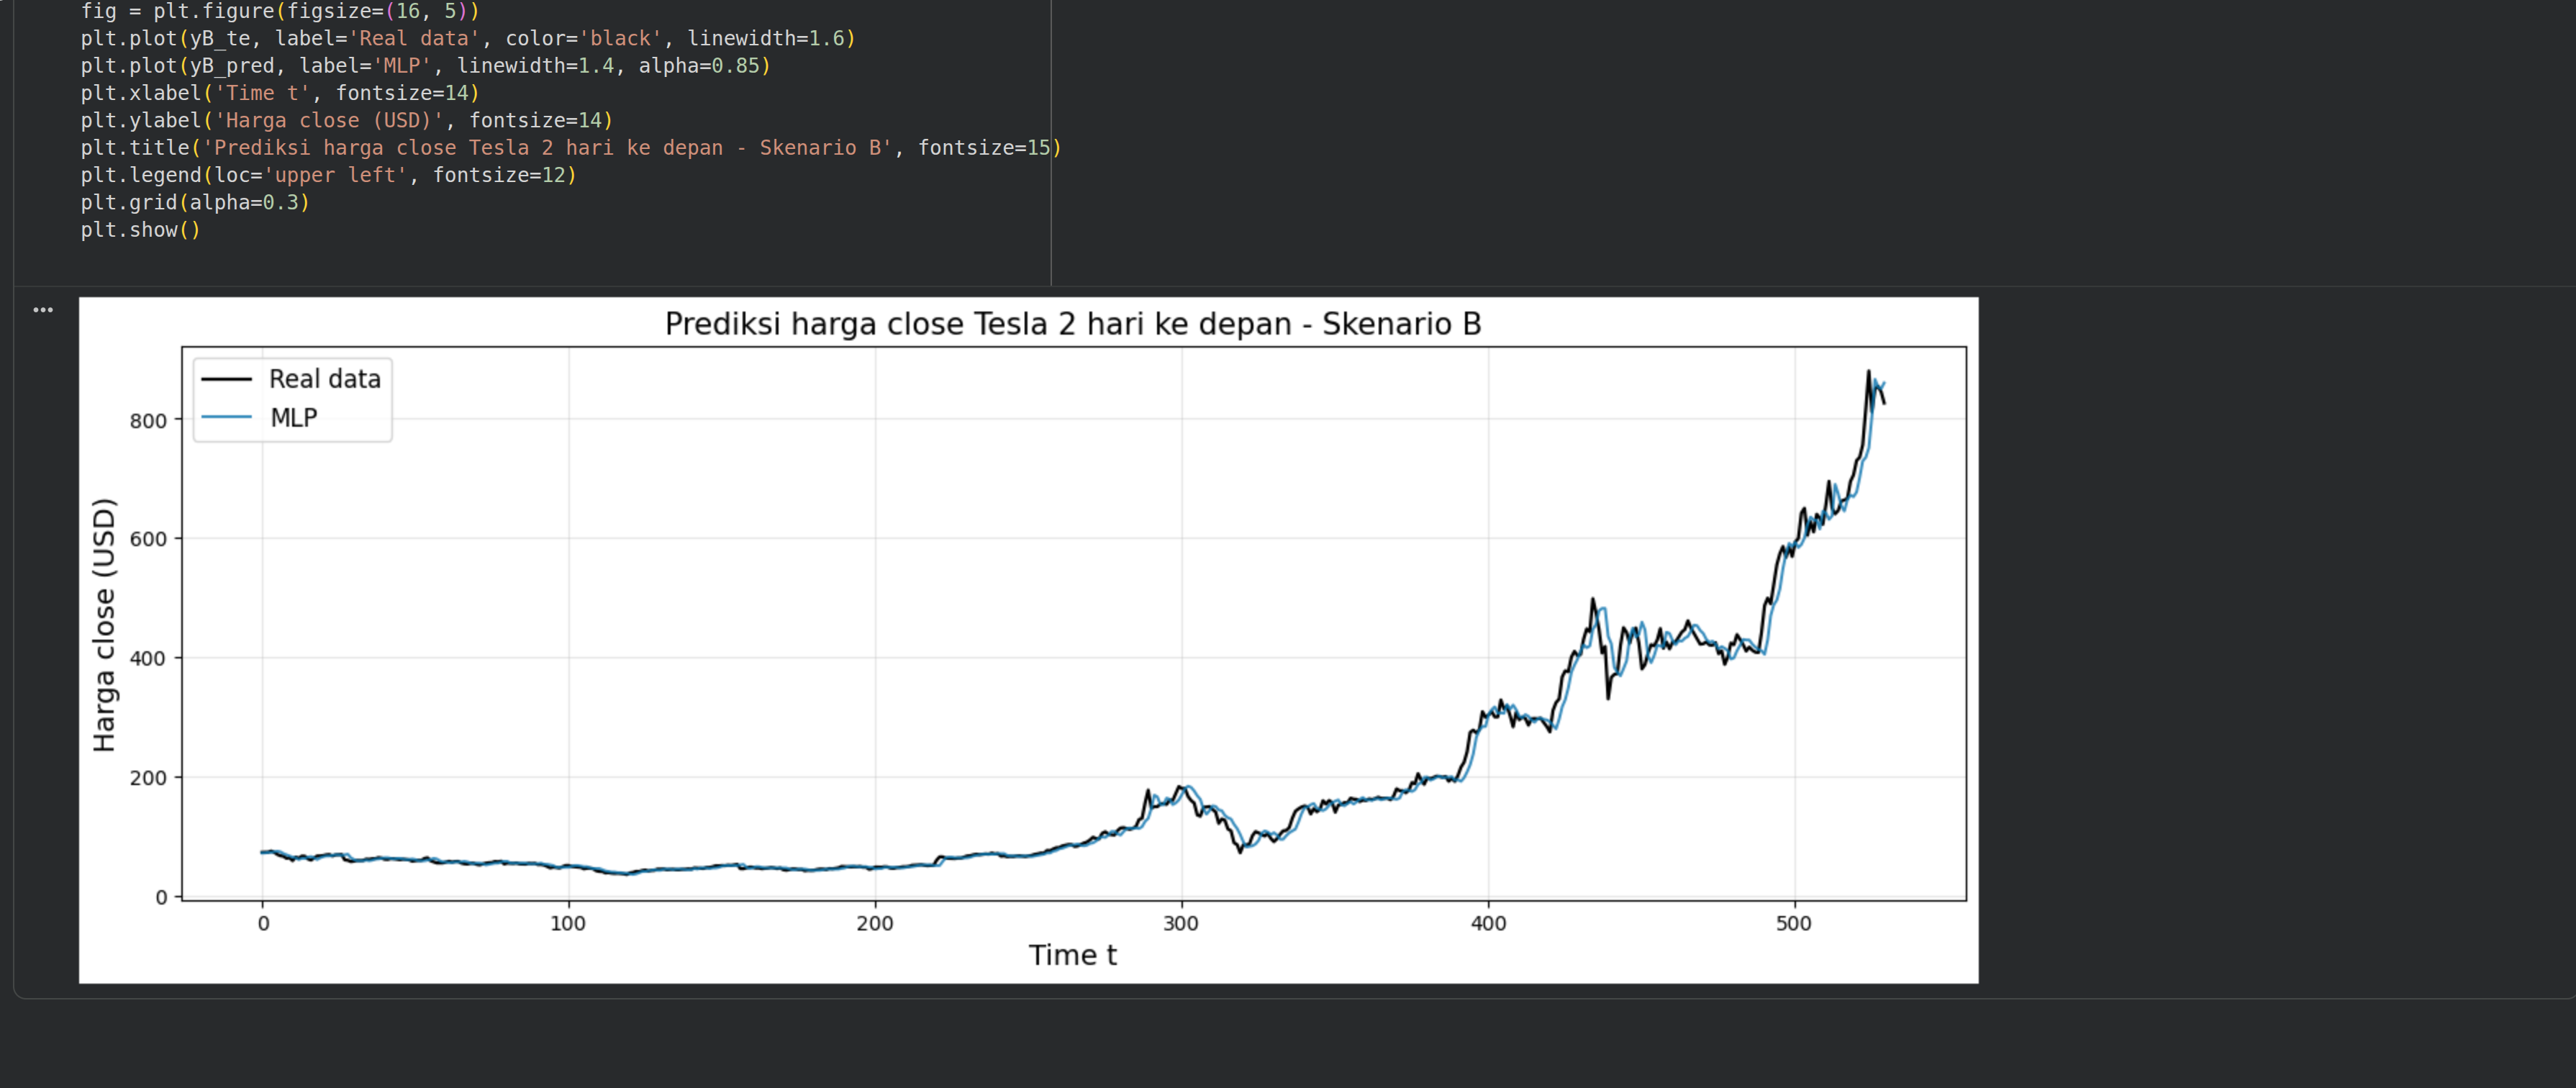
\includegraphics[width=0.98\textwidth]{images/t10-tesla-pred.png}}
\caption{Perbandingan nilai aktual dan prediksi MLP pada Skenario B. MLP mampu mengikuti tren naik harga, sedangkan model berbasis pohon berhenti di sekitar 75 dolar.}
\label{fig:tesla-prediksi}
\end{figure}

\subsection{Perbandingan Skenario A dan B}
Penambahan \texttt{Open} sebagai fitur hanya mengubah hasil sedikit. Pada MLP, RMSE turun dari 18,766 menjadi 18,010 dan Pearson naik tipis dari 0,995 menjadi 0,996. Pada model lain perubahannya bahkan lebih kecil. Ini masuk akal karena harga pembukaan dan harga penutupan Tesla punya korelasi 0,9992, hampir sempurna. Harga \texttt{Open} hampir tidak menambah informasi baru di luar apa yang sudah dibawa \texttt{Close}. Jadi untuk kasus ini, menambah fitur tidak banyak menolong, dan model dengan masukan lebih sedikit sudah cukup.

\clearpage

\chapter{Kesimpulan}
Berdasarkan praktikum yang telah saya lakukan pada Pertemuan 5, saya memahami beberapa hal berikut:
\begin{enumerate}
    \item \textit{Forecasting} adalah proses memperkirakan nilai masa depan dari pola data masa lalu. Untuk data deret waktu, urutan data harus dijaga saat pembagian latih dan uji, sehingga \texttt{shuffle=False} dipakai agar model tidak melihat masa depan.
    \item Saya berhasil mengubah deret waktu menjadi format \textit{supervised learning} dengan teknik \textit{sliding window}, memakai tujuh nilai sebelumnya sebagai masukan. Penambahan delapan fitur statistik (min, max, selisih, mean, std, median, kurtosis, skewness) menaikkan jumlah fitur dari 7 menjadi 15 dan memberi model gambaran distribusi tiap jendela.
    \item Pada percobaan bike sharing, MLP menjadi model terbaik dengan RMSE 1190,549 dan Pearson 0,778, diikuti Random Forest (RMSE 1324,452, Pearson 0,716) dan KNN (RMSE 1357,710, Pearson 0,696). Decision Tree terlemah dari sisi Pearson (0,484) karena pohon tunggal mudah \textit{overfitting}, dan SVR memberi RMSE tertinggi (2404,928) karena fitur tidak dinormalisasi. Baseline naif menghasilkan RMSE 1290,766, sehingga keunggulan MLP di sini nyata tetapi tidak besar.
    \item Pada tugas Tesla, saya membangun dua model: prediksi \texttt{Close} dua hari ke depan dari \texttt{Close} saja, dan dari \texttt{Close} ditambah \texttt{Open}. Hasilnya MLP unggul jauh pada kedua skenario (RMSE 18,766 dan 18,010). Setelah saya telusuri, penyebabnya adalah data uji berisi periode harga yang belum pernah dilihat model saat latihan: 51,1\% nilai uji berada di atas harga tertinggi data latih. Model berbasis pohon dan KNN tidak bisa memprediksi di luar rentang data latihnya, sedangkan MLP bisa mengikuti tren naik. Baseline naif (RMSE 17,278) bahkan sedikit lebih baik dari MLP, tanda bahwa akurasi di sini banyak ditopang oleh sifat harga saham yang bergerak mulus.
    \item Saya memahami bahwa RMSE dan Pearson harus dibaca bersama. RMSE menunjukkan besar kesalahan, sedangkan Pearson menunjukkan seberapa mirip pola prediksi dengan pola aktual. Nilai RMSE yang rendah belum tentu berarti model menangkap pola yang sulit, seperti terlihat pada kasus Tesla.
    \item Saya juga belajar bahwa menambah fitur tidak selalu menolong. Menambahkan \texttt{Open} hanya memperbaiki hasil sedikit karena korelasinya dengan \texttt{Close} hampir sempurna (0,9992), sehingga informasinya sebagian besar sudah terwakili.
\end{enumerate}

\clearpage
\addcontentsline{toc}{chapter}{Daftar Pustaka}
\renewcommand{\bibname}{Daftar Pustaka}
\begin{thebibliography}{99}
    \bibitem{retnoningsih2020} E. Retnoningsih and A. Pramudita, ``Mengenal Machine Learning Dengan Teknik Supervised dan Unsupervised Learning Menggunakan Python,'' \textit{BINA INSANI ICT Journal}, pp. 156--165, 2020.

    \bibitem{santoso2021} A. Santoso, H. Abijono, and D. Anggreini, ``Algoritma Supervised Learning dan Unsupervised Learning dalam Pengolahan Data,'' \textit{Jurnal Teknologi Terapan}, pp. 315--318, 2021.

    \bibitem{vimala2022} T. Vimala and S. Nugroho, ``Forecasting Penjualan Obat Menggunakan Metode Single, Double, dan Triple Exponential Smoothing (Studi Kasus: Apotek Mandiri Medika),'' \textit{Jurnal Penerapan Teknologi Informasi dan Komunikasi}, pp. 90--99, 2022.

    \bibitem{hyndman2021} R. J. Hyndman and G. Athanasopoulos, \textit{Forecasting: Principles and Practice}, 3rd ed. Melbourne, Australia: OTexts, 2021. [Online]. Tersedia: \url{https://web.archive.org/web/2024/https://otexts.com/fpp3/}.

    \bibitem{chai2014} T. Chai and R. R. Draxler, ``Root mean square error (RMSE) or mean absolute error (MAE)? Arguments against avoiding RMSE in the literature,'' \textit{Geoscientific Model Development}, vol. 7, no. 3, pp. 1247--1250, 2014. [Online]. Tersedia: \url{https://doi.org/10.5194/gmd-7-1247-2014}.

    \bibitem{benesty2009} J. Benesty, J. Chen, Y. Huang, and I. Cohen, ``Pearson Correlation Coefficient,'' in \textit{Noise Reduction in Speech Processing}, Berlin, Heidelberg: Springer, 2009, pp. 1--4. [Online]. Tersedia: \url{https://doi.org/10.1007/978-3-642-00296-0_5}.

    \bibitem{sklearn-mlp} Scikit-learn Developers, ``sklearn.neural\_network.MLPRegressor.'' [Online]. Tersedia: \url{https://scikit-learn.org/stable/modules/generated/sklearn.neural_network.MLPRegressor.html}.

    \bibitem{sklearn-knn} Scikit-learn Developers, ``sklearn.neighbors.KNeighborsRegressor.'' [Online]. Tersedia: \url{https://scikit-learn.org/stable/modules/generated/sklearn.neighbors.KNeighborsRegressor.html}.

    \bibitem{sklearn-tree} Scikit-learn Developers, ``sklearn.tree.DecisionTreeRegressor.'' [Online]. Tersedia: \url{https://scikit-learn.org/stable/modules/generated/sklearn.tree.DecisionTreeRegressor.html}.

    \bibitem{sklearn-svr} Scikit-learn Developers, ``sklearn.svm.SVR.'' [Online]. Tersedia: \url{https://scikit-learn.org/stable/modules/generated/sklearn.svm.SVR.html}.

    \bibitem{sklearn-ensemble} Scikit-learn Developers, ``sklearn.ensemble.RandomForestRegressor.'' [Online]. Tersedia: \url{https://scikit-learn.org/stable/modules/generated/sklearn.ensemble.RandomForestRegressor.html}.

    \bibitem{sklearn-metrics} Scikit-learn Developers, ``Metrics and scoring: quantifying the quality of predictions.'' [Online]. Tersedia: \url{https://scikit-learn.org/stable/modules/model_evaluation.html}.

    \bibitem{sklearn-preprocessing} Scikit-learn Developers, ``Preprocessing data.'' [Online]. Tersedia: \url{https://scikit-learn.org/stable/modules/preprocessing.html}.

    \bibitem{sklearn-split} Scikit-learn Developers, ``sklearn.model\_selection.train\_test\_split.'' [Online]. Tersedia: \url{https://scikit-learn.org/stable/modules/generated/sklearn.model_selection.train_test_split.html}.

    \bibitem{pandas-docs} The pandas Development Team, ``pandas.read\_csv.'' [Online]. Tersedia: \url{https://pandas.pydata.org/docs/reference/api/pandas.read_csv.html}.

    \bibitem{numpy-docs} NumPy Developers, ``numpy.array.'' [Online]. Tersedia: \url{https://numpy.org/doc/stable/reference/generated/numpy.array.html}.

    \bibitem{scipy-pearson} SciPy Developers, ``scipy.stats.pearsonr.'' [Online]. Tersedia: \url{https://docs.scipy.org/doc/scipy/reference/generated/scipy.stats.pearsonr.html}.

    \bibitem{scipy-kurtosis} SciPy Developers, ``scipy.stats.kurtosis.'' [Online]. Tersedia: \url{https://docs.scipy.org/doc/scipy/reference/generated/scipy.stats.kurtosis.html}.

    \bibitem{scipy-skew} SciPy Developers, ``scipy.stats.skew.'' [Online]. Tersedia: \url{https://docs.scipy.org/doc/scipy/reference/generated/scipy.stats.skew.html}.

    \bibitem{matplotlib-docs} Matplotlib Development Team, ``Matplotlib Documentation.'' [Online]. Tersedia: \url{https://matplotlib.org/stable/index.html}.

    \bibitem{seaborn-docs} M. Waskom, ``seaborn: statistical data visualization.'' [Online]. Tersedia: \url{https://seaborn.pydata.org/}.

    \bibitem{python-docs} Python Software Foundation, ``Python 3 Documentation.'' [Online]. Tersedia: \url{https://www.python.org/doc/}.

    \bibitem{wikipedia-mlp} Wikipedia, ``Multilayer perceptron.'' [Online]. Tersedia: \url{https://en.wikipedia.org/wiki/Multilayer_perceptron}.

    \bibitem{wikipedia-knn} Wikipedia, ``k-nearest neighbors algorithm.'' [Online]. Tersedia: \url{https://en.wikipedia.org/wiki/K-nearest_neighbors_algorithm}.

    \bibitem{wikipedia-dt} Wikipedia, ``Decision tree learning.'' [Online]. Tersedia: \url{https://en.wikipedia.org/wiki/Decision_tree_learning}.

    \bibitem{wikipedia-svm} Wikipedia, ``Support vector machine.'' [Online]. Tersedia: \url{https://en.wikipedia.org/wiki/Support_vector_machine}.

    \bibitem{wikipedia-rf} Wikipedia, ``Random forest.'' [Online]. Tersedia: \url{https://en.wikipedia.org/wiki/Random_forest}.

    \bibitem{wikipedia-sliding} Wikipedia, ``Sliding window.'' [Online]. Tersedia: \url{https://en.wikipedia.org/wiki/Sliding_window}.

    \bibitem{wikipedia-feature} Wikipedia, ``Feature engineering.'' [Online]. Tersedia: \url{https://en.wikipedia.org/wiki/Feature_engineering}.

    \bibitem{wikipedia-supervised} Wikimedia Commons, ``Supervised and unsupervised learning.'' [Online]. Tersedia: \url{https://commons.wikimedia.org/wiki/File:Supervised_and_unsupervised_learning.png}.

    \bibitem{wikipedia-timeseries} Wikipedia, ``Time series.'' [Online]. Tersedia: \url{https://en.wikipedia.org/wiki/Time_series}.

    \bibitem{wikipedia-overfitting} Wikimedia Commons, ``Overfitting.'' [Online]. Tersedia: \url{https://commons.wikimedia.org/wiki/File:Overfitting.svg}.

    \bibitem{colab-notebook} H. R. Prasetya, ``Praktikum 5: Forecasting (notebook).'' Google Colab. [Online]. Tersedia: \url{https://colab.research.google.com/github/hafidzrizqullahprasetya/PPD/blob/main/pertemuan-5/praktikum-5-forecasting.ipynb}.

    \bibitem{kaggle-bike} L. N. Pathi, ``Bike Sharing Dataset.'' Kaggle. [Online]. Tersedia: \url{https://www.kaggle.com/datasets/lakshmi25npathi/bikesharing-dataset}.

    \bibitem{kaggle-tesla} Timoboz, ``Tesla Stock Data from 2010 to 2020.'' Kaggle. [Online]. Tersedia: \url{https://www.kaggle.com/datasets/timoboz/tesla-stock-data-from-2010-to-2020}.

    \bibitem{bike-mirror} G. Alfarizi, ``data\_science\_practice (bikesharing\_day.csv).'' GitHub. [Online]. Tersedia: \url{https://github.com/ganjar87/data_science_practice}.

    \bibitem{tesla-mirror} P. Jain, ``Stock-Prediction-using-different-models (TSLA.CSV).'' GitHub. [Online]. Tersedia: \url{https://github.com/0xpranjal/Stock-Prediction-using-different-models}.

\end{thebibliography}

\end{document}}
\label{fig:knn}